%auto-ignore
%! TEX root = ../Text.tex
\providecommand{\MainFolder}{..}
\documentclass[\MainFolder/Text.tex]{subfiles}
\begin{document}
\chapter{Towards an invariant definition of canonical IBL-operations}
\label{Section:AppEqDefPrCoPr}
\allowdisplaybreaks
\Correct[caption={Change notation},noline]{Change the notation for the pre-Lie algebra product and for the $D$-space!!! I propose $\triangle$ and }
The canonical $\IBL$-operations $\OPQ_{210}$ and $\OPQ_{120}$ on cyclic cochains of an odd symplectic vector space $V$ have been defined in coordinates in \cite{Cieliebak2015}. In Part~I, we used Definition~\ref{Def:CanonicaldIBL}; it takes and gives invariant objects but requires a choice of basis to describe the inner ``trace'' mechanism. Example~\ref{Ex:Canon} shows that an invariant definition can be obtained from the invariant formalism for evaluation of ribbon graphs developed in Appendix~\ref{Section:Appendix} by plugging in the algebraic Schwarz kernel of the identity as a propagator. In this appendix, we ask the following question.
\begin{Question}\label{Q:CanOp}
Do $\OPQ_{210}$ and $\OPQ_{120}$ arise as a combination of some natural operations coming from the structure of Hochschild cochains on $V$ or from odd symplectic geometry? 
\end{Question}
\Add[caption={DONE Gerstenhaber bracket},noline]{Mention that it is, in fact, the Gerstenhaber bracket!}
In Section~\ref{Sec:LieBrHoch}, we define a canonical Lie bracket $[\cdot,\cdot]$ on Hochschild cochains on~$V$ with values in~$V$ (Definition~\ref{Def:CanonLA} and Proposition~\ref{Prop:CanonLA}), which comes from a natural pre-Lie algebra structure which is visualized as grafting of trees (Equation~\eqref{Eq:PreLie}, Figure~\ref{Fig:GraftTrees} and Lemma~\ref{Lem:PreLie}). This is, in fact, the Gerstenhaber bracket from \cite{Gerstenhaber1963}. Next, we use the symplectic form to define the operator~${}^+$ which ``lowers indices'' (Equation~\ref{Eq:ff}) and show that it takes $[\cdot,\cdot]$ to a Lie bracket on cyclic cochains on~$V$ with values in~$\R$ (Definition~\ref{Def:NewProduct} and Proposition~\ref{Prop:NewLieBr}). By writing down everything in coordinates, we show that this Lie bracket is a degree shift of $\OPQ_{210}$ (Proposition~\ref{Prop:EqOfDefCool}). This answers Question~\ref{Q:CanOp} for $\OPQ_{210}$.

In Section~\ref{Sec:CoprNic}, we relate the cobracket $\OPQ_{120}$ to the canonical $\BV$-operator $\BVOpSym$ on ``functions'' on an odd symplectic vector space (Proposition~\ref{Prop:HochCycSym}). We do it by rewriting~$\OPQ_{120}$ in terms of certain double derivative operators on the tensor algebra, which are associated to a given basis (Definition~\ref{Def:DefOfHochOp}). We prove that both definitions are equivalent (Proposition~\ref{Prop:EqCoprod}). The $\BV$-operator $\BVOpSym$ can be defined geometrically (see~\cite{Doubek2018}), and the cobracket $\OPQ_{120}$ is a factorization of an extension of~$\BVOpSym$ to cyclic invariants with respect to the cyclic shuffle product. We do not know whether this characterization determines $\OPQ_{120}$ uniquely, and hence Question~\ref{Q:CanOp} for~$\OPQ_{120}$ remains open (see Questions~\ref{Q:OpenProbBrCo} for a list of related questions). This section was stimulated by a discussion with J.~Pullman and L.~Peksov\'a at a winter school in Srn\'i, 2019.%\Reminder[noline,caption={Non-reduced operations}]{Check that the constructions here defined the non-reduced $\dIBL$-algebra!!}

\section{Bracket and grafting of trees}\label{Sec:LieBrHoch}

Let $V$ be a $\Z$-graded vector space. We define the weight-graded vector spaces
\begin{equation}\label{Eq:DefOfD}
\DSp V \coloneqq \bigoplus_{k=0}^\infty \Hom(V^{\otimes k},V)\quad\text{and}\quad \DSpRed V \coloneqq \bigoplus_{k=1}^\infty \Hom(V^{\otimes k},V),
\end{equation}
where $\Hom$ denotes the graded vector space generated by homogenous morphisms. The latter space is the weight-reduced version of the former (see Definition~\ref{Def:Grading}).

For homogenous $\psi_1 \in \Hom(V^{\otimes k_1},V)$, $\psi_2 \in \Hom(V^{\otimes k_2},V)$ with $k_1$, $k_2\in\N$ and vectors $v_1$, $\dotsc$, $v_{k_1+k_2-1}\in V$, we define\footnote{If $k_1 = 0$ or $k_2 = 0$, we define $\Star$ to be $0$.}
\begin{equation}\label{Eq:PreLie}
\begin{aligned}
&(\psi_1 \OpPre \psi_2)(v_1 \dotsb v_{k_1 + k_2 -1}) \\
&\ \coloneqq \begin{multlined}[t]\sum_{i=1}^{k_1} (-1)^{\psi_2(v_1 + \dotsb + v_{i-1})}\psi_1(v_1\dotsb v_{i-1} \psi_2(v_i \dotsb v_{k_2 + i -1}) v_{k_2+i} \dotsb v_{k_1 + k_2 - 1}).\end{multlined}
\end{aligned}
\end{equation}
Here and almost everywhere in this section, we suppress writing the tensor product. We recall that we use the same symbol $v$ to denote both a homogenous vector and its degree in the exponent. From \eqref{Eq:PreLie}, we get a bilinear operation 
\[ \OpPre: \DSp V\otimes \DSp V \longrightarrow \DSp V, \]
which preserves the degree and decreases the weight by $1$. It can be visualized as grafting of trees (see Figure~\ref{Fig:GraftTrees}).
\begin{figure}
\centering
%auto-ignore
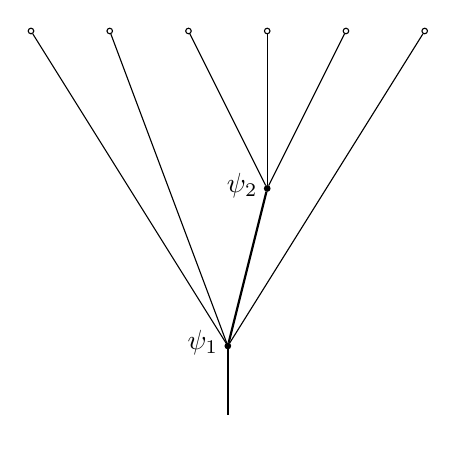
\begin{tikzpicture}
\tikzset{point/.style = {draw, circle, fill=black, minimum size=2pt,inner sep=0pt}}
\def\len{2};
\node[point,label={[left]:$\psi_1$}] (I) at (0,0) {};
\node[point,label={[left]:$\psi_2$}] (II) at (0.5,\len) {};
\node (III) at (0,-.5*\len) {};
\node[point, style={fill=white}] (v1) at (-2.5,2*\len) {};
\node[point, style={fill=white}] (v2) at (-1.5,2*\len) {};
\node[point, style={fill=white}] (v3) at (-.5,2*\len) {};
\node[point, style={fill=white}] (v4) at (.5,2*\len) {};
\node[point, style={fill=white}] (v5) at (1.5,2*\len) {};
\node[point, style={fill=white}] (v6) at (2.5,2*\len) {};
\draw[thick] (I) to (II);
\draw[thick] (I) to (III);
\draw[thin] (I) to (v1);
\draw[thin] (I) to (v2);
\draw[thin] (II) to (v3);
\draw[thin] (II) to (v4);
\draw[thin] (II) to (v5);
\draw[thin] (I) to (v6);
\end{tikzpicture}
\caption{The Gerstenhaber bracket as grafting of trees.}
\label{Fig:GraftTrees}
\end{figure}
\begin{Lemma}[Pre-Lie algebra]\label{Lem:PreLie}\Reminder[noline,caption={Non-reduced pre-Lie algebra.}]{Can one define $\Star$ differently when there are no inputs and get something non-trivial?}
Let $V$ be a graded vector space. The pair $(\DSp V,\OpPre)$ is a graded pre-Lie algebra with respect to the degree, i.e., it holds
\[ (\psi_1 \OpPre \psi_2)\OpPre\psi_3 -  \psi_1 \OpPre (\psi_2\OpPre\psi_3) = (-1)^{\psi_2 \psi_3}\bigl[(\psi_1 \OpPre \psi_3)\OpPre\psi_2 - \psi_1 \OpPre (\psi_3\OpPre\psi_2)\bigr] \]
for all homogenous $\psi_1$, $\psi_2$, $\psi_3 \in \DSp V$. 
\end{Lemma}
\begin{proof}
In the following computations, $U$ denotes a tensor product of homogenous vectors from the vector space~$V$ and $U_i$ denotes a part of a decomposition of $V$, i.e., $U = U_1 \dotsb U_k$. We compute schematically
\begin{align*}
&\bigl((\psi_1 \OpPre \psi_2)\OpPre \psi_3\bigr)(U)  =\begin{aligned}[t]
&\sum (-1)^{\psi_3(U_1 + U_2 + U_3) + \psi_2 U_1}\psi_1(U_1\psi_2(U_2)U_3\psi_3(U_4)U_5) \\
{}+ &\sum (-1)^{\psi_3 U_1 + \psi_2(U_1 + U_2 + U_3+\psi_3)}\psi_1(U_1\psi_3(U_2)U_3\psi_2(U_4)U_5) \\
{}+ &\sum (-1)^{\psi_3(U_1 + U_2)+ \psi_2 U_1}\psi_1(U_1\psi_2(U_2\psi_3(U_3)U_4)U_5)\end{aligned}
\end{align*}
and
\begin{align*}
\bigl(\psi_1 \OpPre (\psi_2\OpPre \psi_3)\bigr)(U)=\sum (-1)^{(\psi_2 - \psi_3) U_1 + \psi_3 U_2}\psi_1(U_1\psi_2(U_2\psi_3(U_3)U_4)U_5).
\end{align*}
Therefore, we have
\begin{align*}
&\bigl[\bigl((\psi_1 \OpPre \psi_2)\OpPre \psi_3\bigr) - \bigl(\psi_1 \OpPre (\psi_2\OpPre \psi_3)\bigr)\bigr](U) \\
&\qquad\qquad=\begin{aligned}[t]&\sum (-1)^{\psi_3(U_1 + U_2 + U_3) + \psi_2 U_1}\psi_1(U_1\psi_2(U_2)U_3\psi_3(U_4)U_5) \\
{}+ &\sum (-1)^{\psi_3 U_1 + \psi_2(U_1 + U_2 + U_3+\psi_3)}\psi_1(U_1\psi_3(U_2)U_3\psi_2(U_4)U_5)
\end{aligned}\\
&\qquad\qquad=\begin{aligned}[t]
(-1)^{\psi_2 \psi_3}\Bigl[&\sum (-1)^{\psi_2(U_1 + U_2 + U_3) + \psi_3 U_1 }\psi_1(U_1\psi_3(U_2)U_3\psi_2(U_4)U_5) \\
{}+&\sum (-1)^{\psi_2 U_1 + \psi_3(U_1 + U_2 + U_3 + \psi_2)}\psi_1(U_1\psi_2(U_2)U_3\psi_3(U_4)U_5)\Bigr]
\end{aligned}\\
&\qquad\qquad=(-1)^{\psi_2 \psi_3}\bigl[\bigl((\psi_1 \OpPre \psi_3)\OpPre \psi_2\bigr) - \bigl(\psi_1 \OpPre (\psi_3\OpPre \psi_2)\bigr)\bigr](U).
\end{align*}
This finishes the proof.
\end{proof}

\begin{Definition}[Canonical Lie algebra on Hochschild cochains]\label{Def:CanonLA}
Let $V$ be a graded vector space. For all $\psi_1$, $\psi_2 \in \DSp V$, we define the bracket by
\[ [\psi_1, \psi_2] \coloneqq \psi_1 \OpPre \psi_2 - (-1)^{\psi_1 \psi_2} \psi_2 \OpPre \psi_1. \]
It is called the \emph{Gerstenhaber bracket}.
\end{Definition}
\begin{Proposition}[Canonical Lie algebra on Hochschild cochains]\label{Prop:CanonLA}
In the situation of Definition~\ref{Def:CanonLA}, the pair $(\DSp V,[\cdot,\cdot])$ is a graded Lie algebra with bracket $[\cdot,\cdot]$ of degree $0$ and weight $-1$.
\end{Proposition}
\begin{proof}
The proof is standard.
\end{proof}

Let $\langle\cdot,\cdot\rangle: V \otimes V \rightarrow \R$ be a homogenous bilinear form of degree $-n$. This means that
\[ \langle v_1, v_2 \rangle \neq 0\quad\Implies\quad v_1 + v_2 = n. \]
To every $\psi\in \Hom(V^{\otimes k},V)$, we associate $\psi^+\in \Hom(V^{\otimes k + 1},\R)$ defined for all $v_1$, $\dotsc$, $v_{k + 1} \in V$ by the formula
\begin{equation}\label{Eq:ff}
\psi^+(v_1\dotsb v_{k+1}) \coloneqq \langle \psi(v_1 \dotsb v_{k}),v_{k+1}\rangle.
\end{equation}
We define the weight-graded vector spaces
\begin{equation}\label{Eq:DSpPlusDef}
\DSpPlus V \coloneqq \bigoplus_{k=0}^\infty \Hom(V^{\otimes k},\R)\quad\text{and}\quad\DSpPlusRed V \coloneqq \bigoplus_{k=1}^\infty \Hom(V^{\otimes k},\R).
\end{equation}
We use here the cohomological grading convention; i.e., $\psi\in \DSpPlus V$ has degree~$d$ and weight~$k$ if and only if for all homogenous $v_1$, $\dotsc$, $v_k\in V$, the following implication holds:
\[ \psi(v_1 \dotsb v_k) \neq 0 \quad\Implies \quad v_1 + \dotsb + v_k = d. \] 
We say that $\varphi\in \DSp V$ is cyclically symmetric if 
\[ \varphi(v_1 \dotsb v_{k}) = \underbrace{(-1)^{v_{k}(v_1 + \dotsb + v_{k-1})}}_{\eqqcolon\varepsilon(v_1\dotsb v_{k},v_{k} v_1 \dotsb v_{k-1})} \varphi(v_{k} v_1 \dotsb v_{k-1}) \]
for all homogenous $v_1$, $\dotsc$, $v_{k}\in V$. We define the weight-graded vector spaces
\begin{align*}
\DSpPlusCyc V &\coloneqq \{\varphi\in \DSpPlus V \mid \varphi\text{ is cyclically symmetric}\}\quad\text{and} \\
\DSpCyc V &\coloneqq \{\psi \in \DSp V \mid \psi^+ \in \DSpPlusCyc V \},
\end{align*}
and similarly for the reduced versions. Formula \eqref{Eq:ff} defines the following linear maps of weight $+1$:
\begin{equation}\label{Eq:CycDiag}
\begin{tikzcd}
 {}^+: & \DSp V \arrow{r} & \DSpPlusRed V \\
 {}^+\coloneqq \Restr{{}^+}{\DSpCyc V}: & \DSpCyc V \arrow{r}\arrow[hook]{u} & \DSpPlusCycRed V\arrow[hook]{u}
\end{tikzcd}
\end{equation}
This might be related to Remark~\ref{Rem:NWG} about weight-reduced bar complexes.

Because $\DSpPlus V$ has the cohomological grading and~$\DSp V$ the standard grading for homogenous maps, ${}^+$ is not homogenous; instead, it satisfies 
\[\Abs{\psi^+} = n - \Abs{\psi}. \]
It is also useful to note that if $\psi^+(v_1\dotsb v_{k+1})\neq 0$, then
\[ \varepsilon(v_1\dotsb v_{k+1},v_{k+1} v_1 \dotsb v_k) = (-1)^{v_{k+1}(\psi^+ - 1)} = (-1)^{v_{k+1}(\psi - n - 1)}. \]

\begin{Lemma}[Restriction of Lie bracket to cyclic invariants]
Let $V$ be a graded vector space and $\langle \cdot,\cdot\rangle: V\otimes V \rightarrow \R$ a homogenous bilinear form of degree $-n$ which is graded antisymmetric. This means that for all homogenous $v_1$, $v_2\in V$, we have
\[ \langle v_1, v_2 \rangle = (-1)^{1+v_1 v_2}\langle v_2, v_1\rangle. \]
Then the Lie bracket $[\cdot,\cdot]$ on $\DSp V$ satisfies $[\DSpCyc V, \DSpCyc V]\subset\DSpCyc V$, and thus it restricts to the Lie bracket (which we denote by the same symbol) 
\[ [\cdot,\cdot]: \DSpCyc V \otimes \DSpCyc V \longrightarrow \DSpCyc V. \]
\end{Lemma}
\begin{proof}
For any homogenous $v_1$, $\dotsc$, $v_{k_1+k_2} \in V$, we compute
\begin{align*}
&\langle[\psi_1,\psi_2](v_1,\dotsc,v_{k_1+k_2-1}),v_{k_1+k_2}\rangle \\
& = \begin{aligned}[t]
&\sum_{i=1}^{k_1} (-1)^{\psi_2(v_1+\dotsb+v_{i-1})}\langle \psi_1(v_1 \dotsb v_{i-1}\psi_2(v_i \dotsb v_{i+k_2-1}) v_{i+k_2}\dotsb \\ &v_{k_1+k_2-1}), v_{k_1+k_2}\rangle - (-1)^{\psi_1 \psi_2}\sum_{j=1}^{k_2}(-1)^{\psi_1(v_1+\dotsb+v_{j-1})}\langle \psi_2(v_1\dotsb \\
&v_{j-1}\psi_1(v_j\dotsb v_{j+k_1-1})v_{j+k_1}\dotsb v_{k_1+k_2-1})), v_{k_1+k_2}\rangle\end{aligned}\\
& = \begin{aligned}[t]
& (-1)^{v_{k_1+k_2}(v_1 + \dotsb v_{k_1+k_2-1})} \\
& \Bigl[\sum_{i=1}^{k_1-1} (-1)^{\psi_2(v_{k_1+k_2}+v_1+\dotsb+v_{i-1})} \langle \psi_1(v_{k_1+k_2} v_1 \dotsb \psi_2(v_i \dotsb v_{i+k_2-1})\\
& v_{i+k_2}\dotsb v_{k_1+k_2-2}), v_{k_1+k_2-1}\rangle+(-1)^{\psi_2(v_1+\dotsb+v_{k_1-1})+v_{k_1+k_2}\psi_2}\\
&\langle \psi_1(v_{k_1+k_2} v_1\dotsb v_{k_1-1}),\psi_2(v_{k_1}\dotsb v_{k_1+k_2-1})\rangle\\
&- (-1)^{\psi_1 \psi_2}\Bigl(\sum_{j=1}^{k_2-1}(-1)^{\psi_1(v_{k_1+k_2}+v_1+\dotsb+v_{j-1})}\langle \psi_2(v_1\dotsb\psi_1(v_j\dotsb\\
& v_{j+k_1-1})v_{j+k_1}\dotsb v_{k_1+k_2-1})), v_{k_1+k_2}\rangle + (-1)^{\psi_1(v_1+\dotsb+v_{k_2-1})+v_{k_1+k_2}\psi_1} \\
& \langle \psi_2(v_{k_1+k_2} v_1\dotsb v_{k_2-1}),\psi_1(v_{k_2},\dotsb,v_{k_1+k_2-1})\rangle\Bigr)\Bigr].
\end{aligned}
\end{align*}
Using graded antisymmetry, we have for the last summand in square brackets
\begin{align*}
&(-1)^{\psi_1(v_1+\dotsb+v_{k_2-1} + v_{k_1 + k_2})}\langle \psi_2(v_{k_1+k_2} v_1\dotsb v_{k_2-1}),\psi_1(v_{k_2},\dotsb,v_{k_1+k_2-1})\rangle \\
&= \begin{multlined}[t](-1)^{1 + \psi_1 \psi_2 + (\psi_2 + v_{k_1 + k_2}+v_1+\dotsb+v_{k_2-1})(v_{k_2}+ \dotsb + v_{k_1+k_2-1})} \\ 
\langle \psi_1(v_{k_2}\dotsb v_{k_1+k_2-1}),\psi_2(v_{k_1+k_2} v_1 \dotsb v_{k_2-1})\rangle\end{multlined} \\
& = (-1)^{1+\psi_1 \psi_2}\langle\psi_1(\psi_2(v_{k_1 + k_2} v_1 \dotsb v_{k_2-1}) v_{k_2}\dotsb v_{k_1 + k_2 - 2}),v_{k_1 + k_2 - 1}\rangle
\end{align*}
and similarly for the second summand
\begin{align*}
&(-1)^{\psi_2(v_1+\dotsb+v_{k_1-1} + v_{k_1+k_2})}\langle\psi_1(v_{k_1+k_2}v_1\dotsb v_{k_1-1}),\psi_2(v_{k_1}\dotsb v_{k_1+k_2-1})\rangle\\
&=\begin{multlined}
(-1)^{1+\psi_1 \psi_2} \langle \psi_2(\psi_1(v_{k_1+k_2} v_1 \dotsb v_{k_1-1}) v_{k_1} \dotsb v_{k_1+k_2-2}),v_{k_1 + k_2 - 1}\rangle.
\end{multlined}
\end{align*}
Therefore, the square bracket equals
\[ \langle[\psi_1,\psi_2](v_{k_1+k_2} v_1 \dotsb v_{k_1 + k_2 - 2}), v_{k_1 + k_2 -1} \rangle \]
and the lemma is proven.
\end{proof} 

The horizontal arrows in \eqref{Eq:CycDiag} become isomorphisms provided that $\langle \cdot,\cdot \rangle$ is non-degenerate (injectivity) and $V$ is of finite type (surjectivity). Therefore, the following definition is possible.
\Reminder[noline,caption={DONE Nondeg, fintype and $+$}]{Be careful, I used to have here in addition degrees bounded from below and now I don't see why. NO PROBLEM, THE ISSUE DISCUSSED IN A FOOTNOTE LATER.}

\newcommand{\NDeg}{\mathbb{\nu}}
\begin{Definition}[Candidate for $\IBL$-product]\label{Def:NewProduct}
Let $V$ be a graded vector space of finite type, and let $\langle \cdot,\cdot \rangle: V\otimes V \rightarrow \R$ be a non-degenerate homogenous graded antisymmetric bilinear form of degree $-n$. Let $\NDeg$ be a formal symbol of degree $n$ realizing the degree shift by $-n$. We define the operation 
\[ \OPQ^*_{210}: (\DSpPlusCycRed V)[-n] \otimes (\DSpPlusCycRed V)[-n] \longrightarrow (\DSpPlusCycRed V)[-n] \] 
for all $\psi_1$, $\psi_2 \in \DSpCyc V$ by
\[ \OPQ^*_{210}( \NDeg\psi_1^+\otimes \NDeg\psi_2^+) \coloneqq \NDeg[\psi_2,\psi_1]^+. \]
\end{Definition}


\begin{Proposition}[Candidate for $\IBL$-product]\label{Prop:NewLieBr}
In the situation of Definition~\ref{Def:NewProduct}, the pair $((\DSpPlusCycRed V)[-n],\OPQ_{210}^*)$ is a graded Lie algebra with the bracket $\OPQ^*_{210}$ of degree $-2n$ and weight $-2$.
\end{Proposition}
\begin{proof}
As for the degree, we have
\begin{align*}
\Abs{\NDeg [\psi_2,\psi_1]^+} &= n+ \Abs{[\psi_2,\psi_1]^+} \\
&= n - \Abs{[\psi_2,\psi_1]}  + n \\
&= n  - \Abs{\psi_1}  - \Abs{\psi_2} + n\\
&= n + \Abs{\psi_1^+} + \Abs{\psi_2^+} - n \\
& = -n + \Abs{\NDeg \psi_1^+} + \Abs{\NDeg \psi_2^+} - n \\
& = \Abs{\NDeg \psi_1^+} + \Abs{\NDeg \psi_2^+} -2n.
\end{align*}
The weights are clear. As for the graded anticommutativity, we have 
\begin{align*}
\OPQ_{210}^*(\NDeg \psi_2^+ \otimes \NDeg\psi_1^+) &= \NDeg[\psi_1,\psi_2]^+ \\
&= -(-1)^{\psi_1 \psi_2} \NDeg[\psi_2,\psi_1]^+ \\ 
&= -(-1)^{\Abs{\NDeg\psi_1}\Abs{\NDeg\psi_2}} \OPQ_{210}^*(\NDeg \psi_1^+ \otimes \NDeg\psi_2^+),
\end{align*}
where we used that 
\[ \Abs{\NDeg \psi^+} = n + \Abs{\psi^+} = n + n - \Abs{\psi} = 2n - \Abs{\psi}. \] 
From the same reason, the graded Jacobi identity for $\OPQ_{210}^*$ is implied by the graded Jacobi identity for $[\cdot,\cdot]$.
\end{proof}

In the situation of Definition~\ref{Def:NewProduct}, let $(e_i)$ be a basis of $V$, and let $(e^i)$ be the dual basis of $V$ such that $\langle e_i, e^j \rangle= \delta_i^j$. To an index $i$, we will assign the degree of $e_i$, so that, e.g., we can write $(-1)^i$ instead of $(-1)^{e_i}$. We will also use the Einstein summation convention.

We define the coordinates
\begin{align*}
g_{ij} &= \langle e_i,e_j\rangle, \\
g^{ij} &= \langle e^i, e^j\rangle, \\
\psi(e_{i_1}\dotsb e_{i_{k_1}}) &= \psi_{i_1 \dotsb i_{k_1}}^i e_i, \\
\psi^+(e_{i_1}\dotsb e_{i_{k_1+1}}) & = \psi_{i_1 \dotsb i_{k_1 + 1}},
\end{align*}
where $\psi\in\DSp V$ and $\psi^+\in\DSpPlus V$. It holds
\[ g_{ij} = (-1)^{i j + 1} g_{ji}, \quad g^{ij} = (-1)^{ij + 1} g^{ji} \quad \text{and}\quad g_{ik}g^{jk} = \delta_i^j. \] 
Equation \eqref{Eq:ff} is now equivalent to 
\begin{equation}\label{Eq:TransfForm}
\psi^i_{i_1 \dotsb i_{k_1}} g_{i i_{k_1+1}}  = \psi_{i_1\dotsb i_{k_1 + 1}},\quad\text{or to}\quad \psi^i_{i_1\dotsb i_{k_1}} = \psi_{i_1 \dotsb i_{k_1} k} g^{ik}.
\end{equation}
We define the operation $\mu: (\DSpPlusCycRed V)^{\otimes 2} \rightarrow \DSpPlusCycRed V$ for $\varphi_1\in \CycHom(V^{k_1 + 1},\R)$, $\varphi_2\in \CycHom(V^{\otimes k_2 + 1},\R)$ with $k_1$, $k_2\in \N_0$ such that $k_1+k_2 \ge 1$ in coordinates by the formula 
\begin{equation}\label{Eq:CoordFormula}
\mu(\varphi_1 \otimes \varphi_2)_{i_1 \dotsb i_{k_1 + k_2}} \coloneqq\begin{multlined}[t] 
\sum_{i,j}\sum_{c=1}^{k_1 + k_2} \varepsilon(i_1 \dotsb i_{k_1 + k_2},i_c \dotsb i_{c-1})(-1)^{(\varphi_1 - i)j} \\ (-1)^i g^{ij} (\varphi_1)_{i i_c \dotsb i_{c+k_1-1}} (\varphi_2)_{j i_{c+k_1} \dotsb i_{c-1}}.
\end{multlined}
\end{equation}
\Correct[noline, caption={DONE possibly wrong sign}]{There might be a sign mistake in $(-1)^a$ because what is needed is probabaly $(-1)^{e^a}$ which differs by $n$. IT IS CORRECT AS IT IS.}
\Modify[caption={DONE finite type},noline]{One can replace finite dimensional by finite type.}
\begin{Remark}[Comparison to \cite{Cieliebak2015}]\label{Rem:CompToCFL}
In order to compare~$\mu$ from \eqref{Eq:CoordFormula} to~$\mu$ from~\cite[Section~10]{Cieliebak2015} (and to the definition of~$\OPQ_{210}$ from Section~\ref{Sec:Alg3}), we must make the replacements
\[ V\mapsto V[1], \quad  n \mapsto n - 2\quad\text{and}\quad\DSpPlusCycRed V\mapsto \DBCyc V. \]
Then $\OPQ_{210}$ and $\OPQ^*_{210}: (\DBCyc V)[2-n]^{\otimes 2} \rightarrow (\DBCyc V)[2-n]$ clearly have the same degree $2(2-n)$.\footnote{The degree of $\OPQ_{210}$ on tensor powers of $C = \DBCyc V [2-n]$, is obtained from the degree on $\Ext C = \Sym(C[1])$ in Definition~\ref{Def:CanonicaldIBL} by substracting $1$ (and by adding $1$ for the cobracket).} Also, $\varphi_1 j + i j$ is precisely the sign needed to move $j$ over $i_{c}\dotsb i_{c+k_1-1}$. We also recall the identification of $\DBCyc V$ with the weight-graded dual $(\BCyc V)^{\WGD}$ from Remark~\ref{Rem:Identifications} and remind that $\BCyc V$ and $\DBCyc V$ were defined to be weight-reduced in order to ease the terminology and notation (see Definition~\ref{Def:BarComplex}).
%The direct comparison to Definition~\ref{Def:CanonicaldIBL} is also clear.
\Correct[noline,caption={DONE wrong degree}]{The degrees seem wrong. $\OPQ_{210}$ has $-2(n-3)-1$ and... NO PROBLEM.}
\end{Remark}

The equality $\OPQ_{210}^*= \OPQ_{210}$ is obtained from the next proposition (c.f., Remark~\ref{Rem:CompToCFL}).

\begin{Proposition}[Equivalence of definitions of $\IBL$-product]\label{Prop:EqOfDefCool}
Let $V$ be a graded vector space of finite type, and let $\langle \cdot,\cdot\rangle: V\otimes V \rightarrow \R$ be a non-degenerate homogenous graded antisymmetric bilinear form of degree $-n$. Then the operation $\OPQ_{210}^*: (\DSpPlusCyc V)[-n]^{\otimes 2} \rightarrow (\DSpPlusCyc V)[-n]$ defined invariantly in Definition~\ref{Def:NewProduct} is a degree shift of the operation $\mu: (\DSpPlusCycRed V)^{\otimes 2} \rightarrow \DSpPlusCycRed V$ defined in coordinates above. More precisely, for all $\varphi_1$, $\varphi_2 \in \DSpPlusCycRed V$, it holds
\[ \OPQ_{210}^*(\NDeg^2 \varphi_1 \otimes \varphi_2) = \NDeg \mu(\varphi_1 \otimes \varphi_2)\qquad\text{in }(\DSpPlusCycRed V)[-n].\]
\end{Proposition}
\begin{proof}
Consider $\psi_1$, $\psi_2 \in \DSpCyc V$ with $k_1$, $k_2$ inputs, respectively. Writing the definition of $[\cdot,\cdot]$ in coordinates, we get 
\begin{align*}
&[\psi_1,\psi_2]^i_{i_1 \dotsb i_{k_1 + k_2-1}} \\
&\qquad=\begin{aligned}[t]
&\sum_{j=1}^{k_1} (-1)^{\psi_2(i_1 + \dotsb + i_{j-1})}(\psi_1)^i_{i_{1} \dotsb i_{j-1} k i_{j+k_2} \dotsb i_{k_1 + k_2 -1}} (\psi_2)^k_{i_{j} \dotsb i_{j+k_2 - 1}} \\ {}+&\sum_{j=1}^{k_2} (-1)^{\psi_1(i_1 + \dotsb + i_{j-1} + \psi_2) + 1}(\psi_2)^i_{i_{1} \dotsb i_{j-1} k i_{j+k_1} \dotsb i_{k_1 + k_2 -1}} (\psi_1)^k_{i_{j} \dotsb i_{j+k_1 - 1}}.
\end{aligned}
\end{align*}
Using \eqref{Eq:TransfForm} and the cyclic symmetry of $\psi_1^+$ and $\psi_2^+$, we compute
\begin{align*}
&[\psi_1,\psi_2]_{i_1 \dotsb i_{k_1 + k_2}} \\ 
&= [\psi_1,\psi_2]^i_{i_1 \dotsb i_{k_1 + k_2 -1}}g_{i i_{k_1 + k_2}}  \\
&=\begin{aligned}[t]
&\sum_{j=1}^{k_1} (-1)^{\psi_2(i_1 + \dotsb + i_{j-1})} (\psi_1)_{i_1 \dotsc i_{j-1} k i_{j+k_2} \dotsc i_{k_1 + k_2}} (\psi_2)^k_{i_j \dotsc i_{j+k_2-1}} \\
+ &\sum_{j=1}^{k_2} (-1)^{\psi_1(i_1 + \dotsb + i_{j-1}+\psi_2)+1} (\psi_2)_{i_1 \dotsc i_{j-1} k i_{j+k_1} \dotsc i_{k_1 + k_2}} (\psi_1)^k_{i_j \dotsc i_{j+k_1-1}}
\end{aligned}\\
& = \begin{aligned}[t] &\sum_{j=1}^{k_1} (-1)^{\psi_2(i_1 + \dotsb + i_{j-1})} g^{ab}(\psi_1)_{i_1 \dotsc i_{j-1} a i_{j+k_2} \dotsc i_{k_1 + k_2}} (\psi_2)_{i_j \dotsc i_{j+k_2-1} b} \\
+&\sum_{j=1}^{k_2} (-1)^{\psi_1(i_1 + \dotsb + i_{j-1} + \psi_2)+1} g^{ab} (\psi_2)_{i_1 \dotsc i_{j-1} a i_{j+k_1} \dotsc i_{k_1 + k_2}} (\psi_1)_{i_j \dotsc i_{j+k_1-1} b}
\end{aligned}\\
& = \begin{aligned}[t]
&\sum_{j=1}^{k_1} \underbrace{(-1)^{\psi_2(i_1+\dotsb+i_{j-1}) + (i_1 + \dotsb + i_{j-1})(\psi_1 - n -1) + b(\psi_2 - n - 1)}}_{\eqqcolon\varepsilon_1} \\
&\qquad g^{ab} (\psi_1)_{a i_{j+k_2}\dotsb i_{k_1+k_2} i_1 \dotsb i_{j-1}}(\psi_2)_{b i_j \dotsb i_{j+k_2-1}}  \\
{}+ & \sum_{j=1}^{k_2} \underbrace{(-1)^{\psi_1(i_1+\dotsb+i_{j-1} + \psi_2) + 1 + (i_1+\dotsb +i_{j-1})(\psi_2 - n - 1) + a(\psi_1-n - 1) + ab + 1}}_{\eqqcolon\varepsilon_2} \\ 
&\qquad g^{ab} (\psi_1)_{a i_j\dotsb i_{j+k_1-1}}
(\psi_2)_{b i_{j+k_1}\dotsb i_{k_1+k_2} i_1 \dotsb i_{j-1}}.
\end{aligned} 
\end{align*}
Notice that the lower indices $i_1$, $\dotsc$, $i_{k_1+k_2}$ appear in cyclic permutations. The first sum consists of cyclic permutation starting with $i_{k_2 + 1}$ and going up to $i_{k_1+k_2+1}$, and the second sum consists of cyclic permutations starting with $i_{1}$ and going up to $i_{k_2}$; hence, all cyclic permutations appear, and it just remains to check the signs. We see that
\begin{align*}
\varepsilon_1 &= (-1)^{\psi_2(i_1+\dotsb+i_{j-1}) + (i_1 + \dotsb + i_{j-1})(\psi_1-n-1) + b(\psi_2 -n- 1)}\\
&=\begin{multlined}[t]\underbrace{(-1)^{(i_1 + \dotsb + i_{j-1} + \psi_2 - n - b)(\psi_1 - n - a + \psi_2 - n - b - 1)}}_{=\varepsilon(i_1\dotsb i_{k_1+k_2}, i_{j+k_2} \dotsb i_{k_1+k_2} i_1 \dotsb i_{j+k_2-1})} (-1)^{b(\psi_1 -n- a)}(-1)^a \\ (-1)^{n(\psi_1 - n) + \psi_2 \psi_1}
\end{multlined}
\end{align*}
and
\begin{align*}
\varepsilon_2 &= (-1)^{\psi_1(i_1+\dotsb+i_{j-1} + \psi_2) + (i_1+\dotsb +i_{j-1})(\psi_2 - n - 1) + a(\psi_1-n-1) + a b} \\
& = \begin{multlined}[t]\underbrace{(-1)^{(i_1 + \dotsb + i_{j-1})(\psi_1 -n - a + \psi_2 -n- b - 1)}}_{=\varepsilon(i_1 \dotsb i_{k_1 + k_2}, i_j \dotsb i_{k_1+k_2} i_1 \dotsb i_{j-1})} (-1)^{b(\psi_1-n-a)}(-1)^a \\
(-1)^{n(\psi_1 - n) + \psi_1 \psi_2 }.
\end{multlined}
\end{align*}
This finishes the proof.
\end{proof}



\section{Cobracket and odd symplectic geometry}\label{Sec:CoprNic}

We start with a remark about the naive dualization of the bracket on the dual.

\begin{Remark}[Naive dualization]
If we ignore the fact that the dualization of spaces like~$\DSp V$ is problematic and we might not get $(\DSp V^{\GD})^{\GD}\simeq \DSp V$,\footnote{It holds $V\simeq (V^{\GD})^{\GD}$ provided that $V$ is of finite type. The tensor product of graded vector spaces of finite type is also of finite type provided that the grading is non-negative. Moreover, one has to require that $W^0 =W^1=0$ for $W$ for which $V=W[1]$ or take suitable completions with respect to weights in order to deal with arbitrary long tensor products in the same degree in the dual of $\DSp V$.} a naive way to obtain a cobracket $\bar{\delta}: \DSp V\rightarrow\DSp V \otimes\DSp V$ would be to dualize the  canonical bracket $[\cdot,\cdot]^*: \DSp V^{\GD} \otimes \DSp V^{\GD} \rightarrow \DSp V^{\GD}$ from the previous section (replacing $V$ by $V^{\GD}$). Because $w([\cdot,\cdot]^*) = -1$, the dual would have $w(\bar{\delta}) = 1$, where $w$ denotes the weights. However, the $\IBL$-cobracket has $w(\OPQ_{120})=-2$ (see Definition~\ref{Def:CanonicaldIBL}), and hence 
\[w\bigl(\bigl(({}^+)^{-1}\otimes({}^+\bigr)^{-1}\bigr)\circ\OPQ_{120}\circ{}^+\bigr) = w(\OPQ_{120}) - 1 = - 3 \neq 1 = w(\bar{\delta}), \]
where the map ${}^+: \DSp V\rightarrow\DSpPlus V$ of weight $+1$ was defined in \eqref{Eq:CycDiag}. It might be interesting to write down the coordinate expression for such $\bar{\delta}$ which comes from~$\OPQ_{120}$ and study its origin and properties on~$\DSp V$.
\end{Remark}

In the following definition, we will use the terms ``cobracket'' and ``$\BV$-operator'' to denote some operations without actually knowing that they satisfy the corresponding relations (see Questions~\ref{Q:OpenProbBrCo} at the end of this section).
 
\begin{Definition}[Hochschild cobracket and $\BV$-operator]\label{Def:DefOfHochOp}
Let $V$ be a graded vector space, let $(e_i)\in V$ be its homogenous basis, and let $(\eta^i)\subset V^{\GD}$ be the dual basis, i.e., it holds $\eta^i(e_j) = \delta^i_j$. We denote by~$\Ten(V^{\GD})$ the tensor algebra over~$V^{\GD}$ and consider its basis $\eta^{\otimes I} \coloneqq \eta^{i_1} \otimes \dotsb \otimes \eta^{i_k}$ for all multiindices $I = (i_1,\dotsc,i_k)$.

For each $i$, $j$, we define the \emph{cyclic double derivative} $\Der_{ij}:\Ten(V^{\GD}) \longrightarrow \Ten(V^{\GD}) \otimes \Ten(V^{\GD})$ on the basis by the following formula, which we explain below:
\begin{equation}\label{Eq:DoubleDeriv}
\Der_{ij}(\eta^{\otimes I}) \coloneqq \sum_{(i,j)\in I} \sum_{\substack{c_1 \in \CycPerm_{k_1}\\ c_2 \in \CycPerm_{k_2}}}\frac{1}{k_1}\frac{1}{k_2}\varepsilon(I,ijI_1^{c_1}I_2^{c_2}) \bigl(\eta^{\otimes I_1^{c_1}} \otimes \eta^{\otimes I_2^{c_2}}\bigr)
\end{equation}
The first sum is over all pairs of indices $(i,j)$ at two distinct positions in $I$. We consider the cyclic order on positions in $I$ (of length $k$) starting from the left and define~$I_1$ and~$I_2$ as the substrings between~$i$ and~$j$ (of length~$k_1$) and between~$j$ and~$i$ (of length~$k_2$), respectively. We include neither $i$ nor $j$ in $I_1$ or $I_2$, i.e., $k= k_1 + k_2 + 2$. The second sum is an average over all cyclic permutations $c_1$ and $c_2$ of $I_1$ and $I_2$, respectively. As usual, $\varepsilon$ stands for the Koszul sign and $i$ has the degree of $e_i$. If $k_1$ or $k_2$ vanishes, we replace the average over $c_1$ or $c_2$, respectively, by $1$ and set $\eta^{\emptyset} = 1$.
%Algorithmically, we take the derivatives with respect to $\eta^i$ and $\eta^j$ with Koszul signs (the derivative acts from the left which is indicated by the arrow), remember positions where they were applied, rotate the whole string to position~$I_1 I_2$, add $\otimes$ in between and permute~$I_1$ and~$I_2$.

On $\Ten(V^{\GD})$, we consider the \emph{shuffle product} $\ProdSh: \Ten(V^{\GD})\otimes\Ten(V^{\GD}) \rightarrow \Ten(V^{\GD})$ which is defined by
\[ \ProdSh(\eta^{\otimes I_1},\eta^{\otimes I_2}) \coloneqq  \sum_{\mu\in\Perm_{k_1,k_2}} \frac{k_1! k_2!}{(k_1 + k_2)!} \varepsilon(I_1 I_2, \mu(I_1 I_2)) \eta^{\otimes\mu(I_1 I_2)}, \]
where $k_1$ and $k_2$ are the lengths of $I_1$ and $I_2$, respectively, and $\Perm_{k_1,k_2}$ denotes the shuffle permutations.

If $V$ is of finite type and $\langle\cdot,\cdot\rangle$ is a non-degenerate homogenous bilinear form on~$V$, we consider the coordinates $g^{ij} = \langle e^i,e^j\rangle$, where $(e^i)\subset V$ is the basis such that $\langle e^i,e_j\rangle = \delta^i_j$. We define the \emph{Hochschild cobracket} $\CoProdHoch: \Ten(V^{\GD}) \rightarrow \Ten(V^{\GD}) \otimes \Ten(V^{\GD})$ by
\begin{equation}
\CoProdHoch = \frac{1}{2}\sum_{i,j} (-1)^{e_i} g^{ij} \Der_{ij}
\end{equation}
and the \emph{Hochschild $\BV$-operator} $\BVOpHoch: \Ten(V^{\GD}) \rightarrow \Ten(V^{\GD})$ by
\begin{equation}
\BVOpHoch \coloneqq \ProdSh \circ \CoProdHoch.
\end{equation}
\end{Definition}

It is easy to check that the definitions of $\ProdSh$, $\CoProdHoch$ and $\BVOpHoch$ do not depend on the choice of the basis $(e_i)$ of $V$.

We denote by~$\Ten(V^{\GD})_{\CycMRM}$ the subspace of cyclic invariants of $\Ten(V^{\GD})$  and by $\Ten(V^{\GD})_{\SymMRM}$ the subspace of symmetric invariants. We consider the cyclization map $\pi_{\CycMRM}: \Ten(V^{\GD}) \rightarrow \Ten(V^{\GD})_{\CycMRM}$ and the symmetrization map $\pi_{\SymMRM}: \Ten(V^{\GD}) \rightarrow \Ten(V^{\GD})_{\SymMRM}$; they are defined by the averages
\begin{align*}
\pi_{\CycMRM}(\eta^{\otimes I})&= \sum_{c\in\CycPerm_k}\frac{1}{k} \varepsilon(I,I^c) \eta^{\otimes I^c}\qquad\text{and}\\
\pi_{\SymMRM}(\eta^{\otimes I}) &= \sum_{\sigma\in\Perm_k}\frac{1}{k!} \varepsilon(I,I^\sigma) \eta^{\otimes I^\sigma},
\end{align*}
respectively, where $k$ is the length of $I$ (if~$k=0$, we have~$\eta^{\emptyset}=1$ and~$\pi_{\CycMRM}(1) \coloneqq 1$). We denote by $\CycCoProj$ the projection to cyclic coinvariants and by $\SymCoProj$ the projection to symmetric coinvariants.

\begin{Definition}[Cyclic and symmetric versions]\label{Def:CycSymVersions}
In the situation of Definition~\ref{Def:DefOfHochOp}, we define the cyclic and symmetric versions of the operations $\Der_{ij}$, $\CoProdHoch$, $\ProdSh$ and $\BVOpHoch$ by precomposing with the inclusions $\CycInc: \Ten(V^{\GD})_{\CycMRM} \rightarrow \Ten(V^{\GD})$ and $\SymInc: \Ten(V^{\GD})_{\SymMRM} \rightarrow \Ten(V^{\GD})$ and postcomposing with the projections $\CycProj: \Ten(V^{\GD}) \rightarrow \Ten(V^{\GD})_{\CycMRM}$ and $\SymProj: \Ten(V^{\GD}) \rightarrow \Ten(V^{\GD})_{\SymMRM}$, respectively. In formulas, we have
\begin{equation}\label{Eq:CycSymVersions}\begin{aligned}
 \DerCyc_{ij} & \coloneqq (\CycProj\otimes\CycProj)\circ\Der_{ij}\circ\CycInc, & \DerSym_{ij} & \coloneqq (\SymProj\otimes\SymProj)\circ\Der_{ij}\circ\SymInc, \\
 \CoProdCyc & \coloneqq (\CycProj\otimes\CycProj)\circ\CoProdHoch\circ\CycInc, &  \CoProdSym & \coloneqq (\SymProj\otimes\SymProj)\circ\CoProdHoch\circ\SymInc, \\ 
 \ProdCyc & \coloneqq \CycProj\circ\ProdSh\circ(\CycInc\otimes\CycInc), & \ProdSym & \coloneqq \SymProj\circ\ProdSh\circ(\SymInc\otimes\SymInc), \\ 
 \BVOpCyc & \coloneqq \CycProj\circ\BVOpHoch\circ\CycInc, & \BVOpSym & \coloneqq \SymProj\circ\BVOpHoch\circ\SymInc.
\end{aligned}\end{equation}
\end{Definition}


\begin{Proposition}[Hochschild, cyclic and symmetric operations]\label{Prop:HochCycSym}
In the situation of Definition~\ref{Def:CycSymVersions}, we consider for every multiindex $I$ the linear functional $\alpha^I: \Ten V \rightarrow\R$ given with respect to the basis $e_{\otimes J}$ by 
\[\alpha^I(e_{\otimes J}) \coloneqq \varepsilon(I,J). \]
We set
\begin{equation*}
\alpha^I_{\mathrm{sym}} = \sum_{\sigma\in \Perm_{k}} \frac{1}{k!} \varepsilon(I,I^\sigma) \alpha^{I^\sigma}\quad\text{and}\quad
\alpha^I_{\mathrm{cyc}} = \sum_{c\in\CycPerm_{k}}\frac{1}{k} \varepsilon(I,I^c)\alpha^{I^c}.
\end{equation*}
We define the monomorphisms $I$, $I_{\CycMRM}$ and $I_{\SymMRM}$ by
\begin{equation}\label{Eq:IdentDiaCycSym}
\begin{tikzcd}[ampersand replacement=\&]
 TV^{\GD} \arrow[hook]{r}{I} \& \DSpPlus V: \& \eta^{\otimes I} \arrow[mapsto]{r} \&  \alpha^I, \\
 (TV^{\GD})_{\CycMRM} \arrow[hook]{r}{I_{\CycMRM}}\arrow[hook]{u} \& \DSpPlusCyc V: \arrow[hook]{u} \& \CycProj(\eta^{\otimes I}) \arrow[mapsto]{r} \& \alpha_{\CycMRM}^I, \\
(TV^{\GD})_{\SymMRM} \arrow[hook]{r}{I_{\SymMRM}}\arrow[hook]{u} \& \DSpPlusSym V: \arrow[hook]{u} \& \SymProj(\eta^{\otimes I}) \arrow[mapsto]{r} \& \alpha_{\SymMRM}^I.
\end{tikzcd}
\end{equation}
The vertical arrows are inclusions and the diagram commutes. Moreover, $I$, $I_{\CycMRM}$ and $I_{\SymMRM}$ become isomorphisms provided that $V$ is of finite type with non-negative degrees. 
%\footnote{We need just $(V^{\otimes k})^{\GD} \simeq {V^{\GD}}^{\otimes k}$.}
In this case, we transfer the operations and obtain the following commutative diagram: 
\begin{equation}\label{Eq:ComDiagram}
\begin{tikzcd}
\BVOpHoch: &\DSpPlus V \arrow{r}{\CoProdHoch} & \DSpPlus V \otimes \DSpPlus V \arrow{r}{\ProdSh} & \DSpPlus V \\
\BVOpCyc: &\DSpPlusCyc V \arrow{r}{\CoProdCyc} \arrow[hook]{u} & \DSpPlusCyc V \otimes \DSpPlusCyc V \arrow{r}{\ProdCyc} \arrow[hook]{u} & \DSpPlusCyc V \arrow[hook]{u} \\
\BVOpSym: & \DSpPlusSym V \arrow{r}{\CoProdSym}\arrow[hook]{u} & \DSpPlusSym V \otimes \DSpPlusSym V \arrow{r}{\ProdSym} \arrow[hook]{u} & \DSpPlusSym V. \arrow[hook]{u}
\end{tikzcd}
\end{equation}
The following formulas hold:
\begin{equation}\label{Eq:CycSymExplicit}
\begin{aligned}
 \CoProdCyc(\alpha^I_{\CycMRM}) &= \frac{1}{2}\sum_{i,j} (-1)^{e_i} g^{ij} \sum_{(i,j)\in I} \varepsilon(I,i j I_1 I_2)(\alpha^{I_1}_{\CycMRM}\otimes \alpha^{I_2}_{\CycMRM}),\\
 \ProdSym(\alpha^{I_1}_{\SymMRM},\alpha^{I_2}_{\SymMRM}) &= \alpha^{I_1 I_2}_{\SymMRM},\\
 \BVOpSym(\alpha^I_{\SymMRM}) &= \frac{1}{2}\sum_{i,j} (-1)^{e_i} g^{ij} \sum_{(i,j)\in I} \varepsilon(I,i j I_1 I_2)\alpha^{I_1 I_2}_{\SymMRM}.
\end{aligned} 
\end{equation}
\end{Proposition}

\begin{proof}
The commutativity of \eqref{Eq:IdentDiaCycSym} is clear from the definitions. The commutativity of~\eqref{Eq:ComDiagram} is equivalent to the commutativity of the same diagram with $\DSpPlus V$, $\DSpPlusCyc V$, $\DSpPlusSym V$ replaced by $\Ten(V^{\GD})$, $\Ten(V^{\GD})_{\CycMRM}$, $\Ten(V^{\GD})_{\SymMRM}$, respectively. This commutativity then follows from the defining relations \eqref{Eq:CycSymVersions} if we show the following inclusions:
\begin{enumerate}[label=(\arabic*)]
\item $\Der_{ij}(\Ten(V^{\GD})_{\CycMRM})\subset\Ten(V^{\GD})_{\CycMRM}\otimes\Ten(V^{\GD})_{\CycMRM}$, 
\item $\Der_{ij}(\Ten(V^{\GD})_{\SymMRM})\subset\Ten(V^{\GD})_{\SymMRM}\otimes\Ten(V^{\GD})_{\SymMRM}$,
\item $\ProdSh(\Ten(V^{\GD})_{\CycMRM}\otimes\Ten(V^{\GD})_{\CycMRM})\subset \Ten(V^{\GD})_{\CycMRM}$,
\item $\ProdSh(\Ten(V^{\GD})_{\SymMRM}\otimes\Ten(V^{\GD})_{\SymMRM})\subset \Ten(V^{\GD})_{\SymMRM}$. 
\end{enumerate}
%follows from commutativity of the diagrams
%\begin{equation}\label{Eq:ComDiagramInv}
%\begin{tikzcd}
%\BVOpHoch: & \Ten(V^{\GD})\arrow{r}{\CoProdHoch}& \Ten(V^{\GD})\otimes\Ten(V^{\GD})\arrow{r}{\ProdSh}& \Ten(V^{\GD}) \\
%\BVOpCyc: &\Ten(V^{\GD})_{\CycMRM} \arrow{r}{\CoProdCyc}\arrow[hook]{u} & \Ten(V^{\GD})_{\CycMRM} \otimes \Ten(V^{\GD})_{\CycMRM}\arrow{r}{\ProdCyc}\arrow[hook]{u}& \Ten(V^{\GD})_{\CycMRM}\arrow[hook]{u} \\
%\BVOpSym: & \Ten(V^{\GD})_{\SymMRM} \arrow{r}{\CoProdSym}\arrow[hook]{u} & \Ten(V^{\GD})_{\SymMRM}  \otimes \Ten(V^{\GD})_{\SymMRM} \arrow{r}{\ProdSym} \arrow[hook]{u} &  \Ten(V^{\GD})_{\SymMRM} \arrow[hook]{u} 
%\end{tikzcd}
%\end{equation}
%and
%\begin{equation}\label{Eq:IdentDiaCycSym}
%\begin{tikzcd}[ampersand replacement=\&]
%(TV^{\GD})_{\SymMRM} \arrow{r}{I_{\SymMRM}}\arrow[hook]{d} \& \DSpPlusSym V \arrow[hook]{d} \\
%(TV^{\GD})_{\CycMRM} \arrow{r}{I_{\CycMRM}}\arrow[hook]{d} \& \DSpPlusCyc V \arrow[hook]{d}\\
% TV^{\GD} \arrow{r}{I} \& \DSpPlus V.
%\end{tikzcd}
%\end{equation}
%where $I_{\SymMRM}$, $I_{\CycMRM}$ and $I$ are given by \eqref{}.
Inclusion (1) is clear from \eqref{Eq:DoubleDeriv}. In fact, it holds even $\Der_{ij}(\Ten(V^{\GD})) \subset  \Ten(V^{\GD})_{\CycMRM} \otimes \Ten(V^{\GD})_{\CycMRM}$. As for inclusion (2), we have
\[ \Der_{ij}\bigl(\pi_{\SymMRM}(\eta^{\otimes I})\bigr) = \sum_{\sigma\in \Perm_k}\frac{1}{k!}\sum_{(i,j)\in I^\sigma}\sum_{\substack{c_1\in\CycPerm_{k_1}\\c_2\in\CycPerm_{k_2}}}\frac{1}{k_1}\frac{1}{k_2}\varepsilon(I,i j I_1^{\sigma c_1}I_2^{\sigma c_2})\eta^{\otimes I_1^{\sigma c_1}}\otimes\eta^{\otimes I_2^{\sigma c_2}}. \]
A pair $(\sigma_1,\sigma_2)\in\Perm_{k_1}\times\Perm_{k_2}$ induces a bijection of the domain of summation, which consists of the elements $\sigma$, $(i,j)$, $c_1$, $c_2$, by keeping $(i,j)$, $c_1$, $c_2$ fixed and defining a new $\tilde{\sigma}$ by altering $\sigma$ to compensate for the effect of $(\sigma_1, \sigma_2)$. The signs fit since we only consider the Koszul sign. Therefore, we have
\[ (\sigma_1\otimes \sigma_2)\Der_{ij}\bigl(\pi_{\SymMRM}(\eta^{\otimes I})\bigr) = \Der_{ij}\bigl(\pi_{\SymMRM}(\eta^{\otimes I})\bigr), \]
and (2) follows. As for (3), we have
\begin{align*}
& \ProdSh\bigl(\CycProj(\eta^{\otimes I_1}),\CycProj(\eta^{\otimes I_2})\bigr)\\
&\qquad= \sum_{\mu\in\Perm_{k_1,k_2}}\frac{k_1!k_2!}{(k_1+k_2)!} \sum_{\substack{c_1\in \CycPerm_{k_1}\\ c_2\in\CycPerm_{k_2}}}\frac{1}{k_1}\frac{1}{k_2}\varepsilon(I_1 I_2,\mu(I_1^{c_1},I_2^{c_2})) \eta^{\otimes \mu(I_1^{c_1},I_2^{c_2})}.
\end{align*}
A permutation $c\in \Perm_k$ again induces a bijection of the domain of summation, which consists of the elements $\mu$, $c_1$, $c_2$. A similar argument holds for (4).

We now derive \eqref{Eq:CycSymExplicit}. Because
\[ \Der_{ij}(\alpha^I_{\CycMRM}) = \sum_{(i,j)\in I} \varepsilon(I,ijI_1I_2) \alpha^{I_1}_{\CycMRM}\otimes\alpha^{I_2}_{\CycMRM}, \]
the formula for $\CoProdCyc$ is clear. As for $\BVOpSym$, because $\ProdSym = \pi_{\SymMRM} \circ \ProdConcat$ for the concatenation product $\ProdConcat(\eta^{\otimes I_1},\eta^{\otimes I_2}) = \eta^{\otimes I_1 I_2}$, we have
\begin{align*}
(\ProdSym\circ \Der_{ij})(\pi_{\SymMRM}\bigl(\eta^{\otimes I})\bigr) & = \sum_{\sigma\in \Perm_k}\frac{1}{k!}\sum_{(i,j)\in I^\sigma}\sum_{\substack{c_1\in\CycPerm_{k_1}\\c_2\in\CycPerm_{k_2}}}\frac{1}{k_1}\frac{1}{k_2}\pi_{\SymMRM}\bigl(\varepsilon(I,i j I_1^{\sigma c_1}I_2^{\sigma c_2})\eta^{\otimes I_1^{\sigma c_1}I_2^{\sigma c_2}}\bigr) \\
& = \sum_{(i,j)\in I} \varepsilon(I,ijI_1 I_2) \pi_{\SymMRM}(\eta^{\otimes I_1 I_2}),
\end{align*}
where we used that $\pi_{\SymMRM} \circ \sigma = \pi_{\SymMRM}$ for every permutation $\sigma$. The formula for $\BVOpSym$ follows. The formula for $\ProdSym$ is also clear.
\end{proof}

%We let \eqref{Eq:DoubleDeriv} descend to cyclic invariants $\Ten(V^{\GD})_{\text{cyc}}$ via the commutative diagram
%\[\begin{tikzcd}
%\dfrac{\vec{\partial}}{\partial \eta^i} \otimes \dfrac{\vec{\partial}}{\partial \eta^j}: &  \Ten(V^{\GD}) \arrow{r} & \Ten(V^{\GD}) \otimes \Ten(V^{\GD}) \arrow[two heads]{d}{\pi_{\text{cyc}}\otimes\pi_{\text{cyc}}}\\
%\Bigl(\dfrac{\vec{\partial}}{\partial \eta^i} \otimes \dfrac{\vec{\partial}}{\partial \eta^j}\Bigr)_{\text{cyc}}: & \Ten(V^{\GD})_{\text{cyc}} \arrow{r}\arrow[hook]{u}{\iota_{\text{cyc}}} & \Ten(V^{\GD})_{\text{cyc}} \otimes \Ten(V^{\GD})_{\text{cyc}},
%\end{tikzcd}\]
%where $\iota_{\text{cyc}}$ is the inclusion and $\pi_{\text{cyc}}$ with $\pi_{\text{cyc}}(\eta^{\otimes I}) = \frac{1}{m}\sum_{c=1}^m \varepsilon(I,I^c) \eta^{\otimes I^c}$ the cyclization map. Recall our convention that the index $i$ has degree of the basis element $e_i$ and that~$I^c$ denotes the $c$-th cyclic permutation of $I$. 
%
%Because the second sum in \eqref{Eq:DoubleDeriv} commutes with cyclic permutations of $I$,  we have
%\begin{equation}\label{Eq:CycVersion}
%\Bigl(\frac{\vec{\partial}}{\partial \eta^i} \otimes \frac{\vec{\partial}}{\partial \eta^j}\Bigr)_{\text{cyc}}\bigl(\alpha^I_{\CycMRM}\bigr) = \sum_{(i,j)\in I} \varepsilon(ijI_1 I_2, I)\alpha^{I_1}_{\CycMRM} \otimes \alpha^{I_2}_{\CycMRM} 
%\end{equation}
%We remind that this expression does not depend on the way we define $\alpha^I$.
%We also consider its cyclic version $\zeta_{\text{cyc}}$ on $(\Ten V/\text{cyc})^{\GD}^{\GD}$, or $\DSpPlusCyc V$, obtained by replacing $\vec{\partial}_i\otimes\vec{\partial}_j$ with $(\vec{\partial}_i\otimes\vec{\partial}_j)_{\text{cyc}}$.
%\begin{Example}[Double derivative is not invariant on all permutations]
%We have 
%\[\Bigl(\frac{\vec{\partial}}{\partial e_1} \otimes \frac{\vec{\partial}}{\partial e_2}\Bigr)(e_1\smallotimes e_2\smallotimes e_3) = (-1)^{e_1 e_2} 1 \otimes e_3\]
%and
%\[\Bigl(\frac{\vec{\partial}}{\partial e_1} \otimes \frac{\vec{\partial}}{\partial e_2}\Bigr)(e_1\smallotimes e_3\smallotimes e_2) = (-1)^{e_2 (e_1+e_3)} e_3 \otimes 1.\]
%These expressions are clearly not equal.
%\end{Example}
%On $\Sym V^{\GD}$, there is the standard commutative associative product $\mu_{\text{sym}}$ (or $\cdot_{\text{sym}}$ in the infix notation). With respect to this product, it holds $\pi(\eta^{\otimes I}) = \eta^{\cdot_{\text{sym}}I}$. If we compose it with $\zeta_{\text{sym}}$, we obtain the unary operator
%\begin{equation}\label{Eq:BVOpMagic}
%\BVOp_{\text{sym}} \coloneqq \mu_{\text{sym}}\circ \zeta_{\text{sym}} = \frac{1}{2}\sum_{i,j=1}^m (-1)^{e_i} g^{ij} \frac{\vec{\partial}}{\partial \eta^i} \cdot \frac{\vec{\partial}}{\partial \eta^j}: \Sym V^{\GD} \longrightarrow \Sym V^{\GD},
%\end{equation}
%where we denoted 
%\[ \frac{\vec{\partial}}{\partial \eta^i} \cdot \frac{\vec{\partial}}{\partial \eta^j} \coloneqq \mu_{\text{sym}}\circ\Bigl(\frac{\vec{\partial}}{\partial \eta^i}\otimes \frac{\vec{\partial}}{\partial \eta^j}\Bigr). \] 
In the formula \eqref{Eq:CycSymExplicit} for $\BVOpSym$, we recognize the canonical $\BV$-operator on $\Sym V^{\GD}$ from~\cite[Definition~4]{Doubek2018}.\footnote{In fact, they work on a bigger ``algebra of functions'' on $V$, which is a completion of $\Sym V^{\GD}$ with respect to a suitable filtration. Their statement is that the algebra of functions on an odd symplectic vector space carries a canonical $\BV$-operator. It is given by the divergence of the Hamiltonian vector field.}
%This is confirmed by the coordinate computation  
%\begin{align*}
%\BVOp_{\text{sym}}(\alpha^I) &= \frac{1}{2} \sum_{i,j=1}^m (-1)^{e_i}g^{ij} \sum_{\sigma\in \Perm_{\Abs{I}}}\frac{1}{\Abs{I}!}\varepsilon(I,I^\sigma)\sum_{(i,j)\in I^\sigma}\varepsilon(i j I_1 I_2,I^\sigma) \bigl(\alpha^{I_1}\cdot_{\text{sym}}\alpha^{I_2}\bigr) \\
%&= \frac{1}{2} \sum_{i,j=1}^m (-1)^{e_i}g^{ij} \sum_{\sigma\in \Perm_{\Abs{I}}}\frac{1}{\Abs{I}!}\varepsilon(I,I^\sigma)\sum_{(i,j)\in I^\sigma}\varepsilon(i j I_1 I_2,I^\sigma)\alpha^{I_1 I_2} \\
%&= \frac{1}{2} \sum_{i,j=1}^m (-1)^{e_i}g^{ij} \sum_{\sigma\in \Perm_{\Abs{I}}}\frac{1}{\Abs{I}!}\varepsilon(I,I^\sigma)\sum_{(i,j)\in I^\sigma}\varepsilon(ijI^\sigma\backslash\{i,j\},I^\sigma)\alpha^{I^\sigma\backslash\{i,j\}} \\
%& =\frac{1}{2} \sum_{(i,j)\in I} (-1)^{e_i}g^{ij} \varepsilon(ij I\backslash\{i,j\},I) \alpha^{I\backslash\{i,j\}}.
%\end{align*}
%The final expression indeed represents a double derivative.
%We remind once more that this expression does not depend on the way we define $\alpha^I$ (see the discussion above).

%\begin{align*}
%(R\otimes R)\Bigl(\frac{\vec{\partial}}{\partial \alpha^i}\otimes \frac{\vec{\partial}}{\partial \alpha^j}\Bigr)_{\SymMRM}(\alpha^I_{\SymMRM})&= \sum_{\sigma\in \Perm_k/\CycPerm_k} \frac{1}{(k-1)!} \varepsilon(I,I^\sigma) 
%\end{align*}
%
%On $\Ten V'/\text{cyc}$, we can consider the bilinear operator $\mu_{\text{cyc}}$ (or $\cdot_{\text{cyc}}$ in the infix notation) defined by
%\[ \mu_{\text{cyc}}\bigl(\alpha^{I_1},\alpha^{I_2}) \coloneqq \sum_{c_1, c_2} \varepsilon(I_1,I_1^{c_1})\varepsilon(I_2,I_2^{c_2})\alpha^{I_1^{c_1}I_2^{c_2}}, \]
%%\[ \mu_{\text{cyc}}\bigl(\pi(\eta^{\otimes I_1}), \pi(\eta^{\otimes I_2}) \coloneqq \sum_{c_1, c_2} \varepsilon(I_1,I_1^{c_1})\varepsilon(I_2,I_2^{c_2})\pi\bigl(\eta^{\otimes I_1^{c_1}}\otimes\eta^{\otimes I_2^{c_2}}\bigr), \]
%where we sum over all cyclic permutations. This product is commutative but not associative (see Example~\ref{Ex:NonAsCyc} below). Similarly as in the symmetric case, we define 
%\[ \BVOp_{\text{cyc}} \coloneqq \mu_{\text{cyc}}\circ \zeta_{\text{cyc}}. \]
%\begin{Example}[Non-associativity of $\cdot_{\text{cyc}}$]\label{Ex:NonAsCyc}
%On $\Ten V / \text{cyc}$, we have
%\begin{align*}
% (e_1\cdot_{\text{cyc}} e_2)\cdot_{\text{cyc}} (e_3 e_4) &= (e_1 e_2)\cdot_{\text{cyc}}(e_3 e_4)\\
% & = \begin{multlined}[t] e_1 e_2 e_3 e_4 + (-1)^{e_1 e_2} e_2 e_1 e_3 e_4 \\ {}+ (-1)^{e_3 e_4} e_1 e_2 e_4 e_3 + (-1)^{e_1 e_2 + e_3 e_4} e_2 e_1 e_4 e_3.\end{multlined}
%\end{align*}
%but
%\begin{align*}
% e_1 \cdot_{\text{cyc}} (e_2 \cdot_{\text{cyc}} (e_3 e_4)) &= e_1 \cdot_{\text{cyc}} \bigl( e_2 e_3 e_4 + (-1)^{e_3 e_4}e_2 e_4 e_3 \bigr) \\
% & = \begin{multlined}[t] 
% e_1 e_2 e_3 e_4 + (-1)^{e_4(e_2 + e_3)} e_1 e_4 e_2 e_3 \\{}+ (-1)^{e_2(e_3 + e_4)} e_1 e_3 e_4 e_2 + (-1)^{e_3 e_4} e_1 e_2 e_4 e_3 \\ {}+ (-1)^{e_3 e_2} e_1 e_3 e_2 e_4 + (-1)^{e_3 e_4 + e_2 e_4 + e_2 e_3} e_1 e_4 e_3 e_2.
%\end{multlined} 
%\end{align*}
%These expressions are not equal, and hence $\cdot_{\text{cyc}}$ is not associative.
%\end{Example}
We will now relate $\zeta_{\text{cyc}}$ to $\OPQ_{120}$. The steps are similar to Section~\ref{Sec:LieBrHoch}. We define the coproduct $\OPQ_{120}^*: (\DSpPlusCyc V)[-n] \rightarrow (\DSpPlusCyc V)[-n]^{\otimes 2}$, where $-n$ is the degree of $\langle\cdot,\cdot\rangle$, by 
\begin{equation}\label{Eq:CoprCandid}
\OPQ_{120}^*(\nu\varphi) = \nu^2\zeta_{\text{cyc}}(\varphi)\qquad\text{for all }\varphi\in \DSpPlusCyc V,
\end{equation}
where $\nu$ is a formal symbol of degree $n$.

For $\varphi\in \CycHom(V^{\otimes k},\R)$ with $k\ge 4$, we define $(\delta\varphi)\in(\DSpPlusCycRed V)^{\otimes 2}$ using the coordinates
\begin{equation}\label{Eq:CoefCoord}
\varphi_{I} \coloneqq \varphi(e_{\otimes I})\quad\text{and}\quad (\delta\varphi)_{I_1;I_2} = (\delta\varphi)(e_{\otimes I_1} \otimes e_{\otimes I_2})
\end{equation}
by
\begin{equation}\label{Eq:StdCoprCoord}
(\delta\varphi)_{I_1;I_2} \coloneqq \sum_{\substack{c_1 \in\CycPerm_{k_1} \\ c_2\in\CycPerm_{k_2}}} \sum_{i,j} (-1)^{e_i}g^{ij} \varepsilon(I_1,I_1^c)\varepsilon(I_2,I_2^c)(-1)^{e_j I_1} \varphi_{i I_1^{c_1} j I_2^{c_2}}.
\end{equation}
We set $\delta \varphi = 0$ for $k\le 3$. In order to obtain $(\delta\varphi)\in(\DSpPlusCycRed V)^{\otimes 2}$, we use the embedding $(\DSpPlusCyc V)^{\otimes k} \subset (\Ten V)^{\otimes k*}$ from Remark~\ref{Rem:Identifications}. Note that we can also use the canonical identification $(\Ten V/\CycMRM)^{\WGD}\simeq \DSpPlusCyc V$ and work with the cyclic words $e_I \coloneqq \CycCoProj(e_{\otimes I})$ instead. We see that~\eqref{Eq:StdCoprCoord} is precisely the defining equation \cite[Equation~(10.6)]{Cieliebak2015} for the $\IBL$-cobracket $\delta: \DSpPlusCycRed V \rightarrow (\DSpPlusCycRed V)^{\otimes 2}$, and $\OPQ_{120}:(\DSpPlusCycRed V)[-n]\rightarrow(\DSpPlusCycRed V)[-n]^{\otimes 2}$ is the degree shift of $\delta$.

The equality $\OPQ_{120}^*= \OPQ_{120}$ on the reduced part
is obtained from the next proposition (c.f., Remark~\ref{Rem:CompToCFL} for the translation from the $\DSpPlusCycRed$- to the  $\DBCyc$-notation).\Modify[caption={DONE finite type},noline]{One can replace finite dimensional by finite type.}
\begin{Proposition}[Equivalence of definitions of $\IBL$-cobracket]\label{Prop:EqCoprod}
Let $V$ be a graded vector space of finite type, and let $\langle\cdot,\cdot\rangle$ be a non-degenerate homogenous bilinear form of degree~$-n$. For every $\varphi\in \DSpPlusCycRed V$, it holds
\[ \OPQ_{120}^*(\nu \varphi) = \nu^2 \delta \varphi\qquad\text{in}\quad(\DSpPlusCycRed V)[-n]^{\otimes 2}. \]
\end{Proposition}
\begin{proof}
%We identify the cyclic invariants of the weight-graded dual $(\Ten V')_{\text{cyc}}$ with the weight-graded dual of cyclic co-invariants $\bigl(\Ten V/\text{cyc}\bigr)''$ so that $\alpha^I$ which corresponds to $\pi_{\text{cyc}}(\eta^{\otimes I}) = \frac{1}{m}\sum_{c=1}^m \varepsilon(\eta,c) \eta^{i_c} \otimes \dotsb \otimes \eta^{i_{c-1}}$ acts on $e_J = \pi(e_{\otimes J})$, where $\pi: \Ten V \rightarrow \Ten V/\mathrm{cyc}$ is the canonical projection, as 
We consider the basis $(\alpha^I_{\CycMRM})$ of $\DSpPlusCyc V$ from Proposition~\ref{Prop:HochCycSym}. Given $\varphi\in\DSpPlusCyc V$, we can write $\varphi=\sum_{I}\frac{1}{\Abs{I}}\varphi_I\alpha^I_{\CycMRM}$, where we sum over all multiindices $I$ and $\varphi_I\in \R$ are coefficients cyclically symmetric in $I$. For every $I$ of length $k$, we have
\[ \varphi(e_{\otimes I}) = \sum_{c\in \CycPerm_k}\frac{1}{k}\varphi_{I^c} \alpha^{I^c}_{\CycMRM}(e_{\otimes I}) = \sum_{c\in\CycPerm_k}\frac{1}{k}\varphi_{I^c} \varepsilon(I^c,I) = \varphi_I, \]
and hence $\varphi_I$ correspond to the coefficients \eqref{Eq:CoefCoord}. Using \eqref{Eq:CycSymExplicit}, we compute
\begin{align*}
 \CoProdCyc(\varphi)&= \frac{1}{2}\sum_I \sum_{(i,j)\in I} \frac{1}{\Abs{I}}\varphi_I  (-1)^{e_i} g^{ij}\varepsilon(I,i j I_1 I_2) \alpha^{I_1}_{\CycMRM} \otimes \alpha^{I_2}_{\CycMRM} \\
 &=\frac{1}{2}\sum_J \sum_{c\in \CycPerm_{\Abs{J}}} \sum_{j \in J\backslash\{j_1\}} \frac{1}{\Abs{J}}\varphi_{J^c} (-1)^{e_{j_1}} g^{{j_1} j}(-1)^{j J_1}\varepsilon(J,J^c) \alpha^{J_1}_{\CycMRM} \otimes \alpha^{J_2}_{\CycMRM} \\
 &=\frac{1}{2}\sum_J\sum_{j\in J\backslash\{j_1\}} \varphi_J(-1)^{e_{j_1}}g^{j_1 j}(-1)^{j J_1} \alpha_{\CycMRM}^{J_1}\otimes \alpha_{\CycMRM}^{J_2}  \\
 & = \sum_{J_1, J_2}\underbrace{\Bigl(\frac{1}{2}\sum_{i,j} (-1)^{e_i} g^{ij}(-1)^{j J_1} \varphi_{i J_1 j J_2} \Bigr)}_{\eqqcolon(*)_{J_1;J_2}}\alpha^{J_1}_{\CycMRM}\otimes\alpha^{J_2}_{\CycMRM}.
\end{align*}
On the second line, we used the bijection of the summation domains consisting of $I$, $(i,j)$, resp.~$J$, $c$, $b$, which assigns to~$I$ its cyclic permutation~$J$ such that the position of~$i$ corresponds to the first position of~$J$, i.e., it holds~$j_1 = i$. On the third line, we used that~$\varphi_I$ are cyclic symmetric, and on the fourth line, we just rewrote the summation using $J = i J_1 j J_2$. We now relate $(*)_{J_1;J_2}$ to $(\delta\varphi)_{J_1;J_2}$. We compute (notice that there is no Koszul sign from the application of the tensor product, c.f., Remark~\ref{Rem:Identifications})
\begin{align*}
\zeta_{\text{cyc}}(\varphi)(e_{I_1}\otimes e_{I_2}) & = \Bigl(\sum_{\substack{c_1\in\CycPerm_{k_1}\\c_2\in\CycPerm_{k_2}}}(*)_{I_1^{c_1};I_2^{c_2}}\alpha_{\CycMRM}^{I_1^{c_1}}\otimes\alpha_{\CycMRM}^{I_2^{c_2}}\Bigr)(e_{I_1}\otimes e_{I_2}) \\
& = \sum_{\substack{c_1\in\CycPerm_{k_1}\\c_2\in\CycPerm_{k_2}}}\varepsilon(I_1^{c_1},I_1)\varepsilon(I_2^{c_2},I_2)(*)_{I_1^{c_1};I_2^{c_2}} \\
& = (\delta\varphi)_{J_1;J_2}.
\end{align*}
This shows the proposition.
\end{proof}

%
%\begin{Proposition}[Factorizations of $\BV$-operators with respect to the product]
%The new operations $\BVOp_{\SymMRM}$, $\BVOp_{\CycMRM}$, $\zeta_{\SymMRM}$ and $\zeta_{\CycMRM}$ fit in the commutative diagram
%\begin{equation}\label{Eq:ComDiagram}
%\begin{tikzcd}
%\BVOp_{\mathrm{sym}}: & \DSpPlusSym V \arrow{r}{\zeta_{\mathrm{sym}}}\arrow[hook]{d} & \DSpPlusSym V \otimes \DSpPlusSym V \arrow{r}{\mu_{\mathrm{sym}}} \arrow[hook]{d} & \DSpPlusSym V \arrow[hook]{d} \\
%\BVOp_{\mathrm{cyc}}: &\DSpPlusCyc V \arrow{r}{\zeta_{\mathrm{sym}}} & \DSpPlusCyc V \otimes \DSpPlusCyc V \arrow{r}{\mu_{\mathrm{cyc}}} & \DSpPlusCyc V.
%\end{tikzcd}
%\end{equation}
%Here $\DSpPlusCyc V$, resp.~$\DSpPlusSym V$ denote the spaces of cyclic symmetric, resp.~symmetric multilinear functionals on $V$ and $\mu_{\CycMRM}$, resp.~$\mu_{\SymMRM}$ the cyclic shuffle product, resp.~the symmetric product. These are induced on $\DSpPlusCyc V$, resp.~$\DSpPlusSym V$ from the corresponding products on coinvariants of $\Ten V'$ via the identification \eqref{Eq:IdDiagram} using the following definitions of $\alpha^I$'s:
%\begin{equation}\label{Eq:NewAlphas}
%\alpha^I_{\mathrm{sym}}(e_{\otimes J}) = \sum_{\sigma\in \Perm_{\Abs{J}}} \frac{1}{\Abs{J}!}\varepsilon(I,J^\sigma)\quad\mathrm{and}\quad \alpha^I_{\mathrm{cyc}}(e_{\otimes J}) = \sum_{c} \frac{1}{\Abs{J}}\varepsilon(I,J^c). 
%\end{equation}
%\end{Proposition}
%\begin{proof}
%For any $I$, $k = \Abs{I}$, we have
%\begin{align*}
%\SymProj(\eta^{\otimes I}) &= \frac{1}{k!}\sum_{\sigma\in\Perm_{k}} \varepsilon(I,I^\sigma) \eta^{\otimes I^\sigma}\\
%&=\frac{1}{(k-1)!} \sum_{\sigma\in\Perm_k/\CycPerm_k} \varepsilon(I,I^{\sigma})\sum_{c} \frac{1}{k}\varepsilon(I^{\sigma},I^{\sigma c})\eta^{\otimes\sigma c} \\
%& = \frac{1}{(k-1)!} \sum_{\sigma\in\Perm_k/\CycPerm_k} \varepsilon(I,I^\sigma)\CycProj(\eta^{\otimes I^\sigma}).
%\end{align*}
%Therefore, the inclusion $(\Ten V')_{\SymMRM} \subset (\Ten V')_{\CycMRM}$ transforms under \eqref{Eq:IdDiagram} with respect to a basis $\alpha^I$ into
%\begin{equation}\label{Eq:MapR}
%R(\alpha^I_{\SymMRM}) \coloneqq \frac{1}{(k-1)!} \sum_{\sigma \in \Perm_k/\CycPerm_k} \varepsilon(I,I^\sigma) \alpha_{\CycMRM}^{I^\sigma}.
%\end{equation}
%Denoting by $I_{\CycMRM}$, resp.~$I_{\SymMRM}$ the maps with codomain $\DSpPlusCyc$, resp.~$\DSpPlusSym$ from \eqref{Eq:IdDiagram}, we have using \eqref{Eq:NewAlphas} for any $J$ the following
%\begin{align*}
% (I_{\CycMRM}\circ R)(\alpha^I_{\SymMRM})(e_J) &= \frac{1}{(k-1)!} \sum_{\sigma\in\Perm_k/\CycPerm_k} \varepsilon(I,I^\sigma)I_{\CycMRM}(\alpha^{I^\sigma}_{\CycMRM})(e_J) \\
% &= \frac{1}{(k-1)!} \sum_{\sigma\in\Perm_k/\CycPerm_k} \varepsilon(I,I^\sigma)\frac{1}{\Abs{J}} \sum_{c} \varepsilon(I^{\sigma},J^c) \\
% & = \frac{1}{k!} \sum_{\sigma\in\Perm_{k}} \varepsilon(I,J^\sigma)\\
% & = I_{\SymMRM}(\alpha^I_{\SymMRM})(e_J).
%\end{align*}
%Therefore, the diagram
%\begin{equation}\label{Eq:IdentDiaCycSym}
%\begin{tikzcd}[ampersand replacement=\&]
%(TV')_{\mathrm{sym}} \arrow{r}{I_{\mathrm{sym}}} \arrow[hook]{d} \& \DSpPlusSym V \arrow[hook]{d} \\
%(TV')_{\mathrm{cyc}} \arrow{r}{I_{\mathrm{cyc}}} \& \DSpPlusCyc V
%\end{tikzcd}
%\end{equation}
%commutes, and we can check \eqref{Eq:ComDiagram} in terms of $\alpha^I$ with $R$ as the vertical map. We compute
%\begin{align*}
%R(\alpha^{I_1}_{\SymMRM})\cdot_{\CycMRM}R(\alpha^{I_2}_{\SymMRM}) &=\begin{multlined}[t]\frac{1}{(k_1-1)!}\frac{1}{(k_2-1)!}\sum_{\substack{\sigma_1\in \Perm_{k_1}/\CycPerm_{k_1} \\ \sigma_2\in \Perm_{k_2}/\CycPerm_{k_2}}} \varepsilon(I_1,I_1^{\sigma_1})\varepsilon(I_2,I_2^{\sigma_2})\frac{1}{k_1}\frac{1}{k_2}\\
%\frac{k_1! k_2!}{(k_1 + k_2)!}\sum_{\substack{\mu\in\Perm_{k_1, k_2}\\c_1, c_2}}\varepsilon(I_1^{\sigma_1}I^{\sigma_2},\mu(I_1^{\sigma_1 c_1}I^{\sigma_2 c_2})) \alpha_{\CycMRM}^{\mu(I_1^{\sigma_1 c_1}I^{\sigma_2 c_2})}\end{multlined} \\
%& = \begin{multlined}[t]\frac{1}{(k_1 + k_2)!} \sum_{\substack{\mu\in \Perm_{k_1,k_2} \\ \sigma_1\in \Perm_{k_1}/\CycPerm_{k_1} \\ \sigma_2\in \Perm_{k_2}/\CycPerm_{k_2} \\ c_1, c_2}}\varepsilon(I_1 I_2, \mu(I_1^{\sigma_1 c_1}I_2^{\sigma_2 c_2}))\alpha_{\CycMRM}^{\mu(I_1^{\sigma_1 c_1}I^{\sigma_2 c_2})}\end{multlined} \\
%& =\begin{multlined}[t]\frac{1}{(k_1+k_2)!} \sum_{\mu\in\Perm_{k_1+k_2}}\varepsilon(I_1 I_2,\mu(I_1 I_2)) \alpha_{\CycMRM}^{\mu(I_1 I_2)}
%\end{multlined}\\
%& = \begin{multlined}[t]
% \frac{1}{(k_1+k_2-1)!} \sum_{\mu\in \Perm_{k_1+k_2}/\CycPerm_{k_1+k_2}}  \varepsilon(I_1 I_2,\mu(I_1 I_2)) \alpha_{\CycMRM}^{\mu(I_1 I_2)}
% \end{multlined}\\
% & = R(\alpha^{I_1 I_2}_{\SymMRM}) \\
% & = R(\alpha^{I_1}_{\SymMRM}\cdot_{\SymMRM}\alpha^{I_2}_{\SymMRM}),
%\end{align*}
%and hence the second square of \eqref{Eq:ComDiagram} commutes. As for the first square, we compute
%\begin{align*}
%& (R\otimes R)\Bigl(\frac{\vec{\partial}}{\partial\eta^i}\otimes\frac{\vec{\partial}}{\partial\eta^j}\Bigr)_{\SymMRM}(\alpha^I_{\SymMRM}) \\
%&\qquad =\begin{multlined}[t]\sum_{\sigma\in \Perm_k / \CycPerm_k} \frac{1}{(k-1)!} \varepsilon(I,I^\sigma) \sum_{(i,j)\in I^\sigma} \varepsilon(i j I_1 I_2, I^\sigma) R(\alpha^{I_1}_{\SymMRM}) \otimes R(\alpha^{I_2}_{\SymMRM})\end{multlined}\\
%&\qquad =\begin{multlined}[t]\sum_{\sigma\in \Perm_k / \CycPerm_k} \frac{1}{(k-1)!} \varepsilon(I,I^\sigma) \sum_{(i,j)\in I^\sigma} \varepsilon(i j I_1 I_2, I^\sigma) \frac{1}{(k_1-1)!}\frac{1}{(k_2-1)!} \\ \sum_{\substack{\mu_1\in\Perm_{k_1}/\CycPerm_{k_1}\\\mu_2\in\Perm_{k_2}/\CycPerm_{k_2}}} \varepsilon(I_1,I_1^{\mu_1}) \varepsilon(I_2,I_2^{\mu_2}) \alpha_{\CycMRM}^{I_1^{\mu_1}} \otimes \alpha_{\CycMRM}^{I_2^{\mu_2}}
%\end{multlined} \\
%&\qquad = \frac{1}{(k-1)!}\frac{1}{(k_1-1)!}\frac{1}{(k_2-1)!}\sum_{\substack{\sigma\in\Perm_k/\CycPerm_k\\\mu_1\in\Perm_{k_1}/\CycPerm_{k_1}\\\mu_2\in\Perm_{k_2}/\CycPerm_{k_2}\\(i,j)\in I^\sigma}} \varepsilon(I,I^\sigma)\varepsilon(I^\sigma,ijI_1^{\mu_1}I_2^{\mu_2})\alpha_{\CycMRM}^{I_1^{\mu_1}} \otimes \alpha_{\CycMRM}^{I_2^{\mu_2}} \\
%&\qquad= \frac{1}{(k-1)!} \sum_{\mu\in\Perm_k/\CycPerm_k} \varepsilon(I,I^\sigma)\sum_{(i,j)\in I^\sigma} \varepsilon(i j I_1 I_2,I^\sigma)\alpha_{\CycMRM}^{I_1}\otimes\alpha_{\CycMRM}^{I_2} \\
%&\qquad = \frac{1}{(k-1)!} \sum_{\sigma\in \Perm_k/\CycPerm_k} \varepsilon(I,I^\sigma)\Bigl(\frac{\vec{\partial}}{\partial \alpha^i} \otimes \frac{\partial}{\partial \alpha^j}\Bigr)_{\CycMRM}(\alpha_{\CycMRM}^{I^\sigma}) \\
%& \qquad = \Bigl(\frac{\vec{\partial}}{\partial \alpha^i} \otimes \frac{\partial}{\partial \alpha^j}\Bigr)_{\CycMRM} R(\alpha^I_{\SymMRM}) 
%\end{align*}
%IT DOES NOT WORK BECAUSE THE ACTION OF $\Perm_{k}^{\CycMRM}$ ON\textsl{•} $\Perm_k$ IS NOT FREE!!!
%\end{proof}
%
%\begin{Remark}[Continuation to Hochschild cochains]
%Both of the squares
%\[\begin{tikzcd}
% V\otimes D^+_{\CycMRM}V \arrow{r}{\mu_{\CycMRM}} & d
%\end{tikzcd}\]
%\begin{align*}
% I_{\CycMRM}(\alpha^I_{\CycMRM})(e_J) = \frac{1}{k}\sum_{c}\varepsilon(I,J^c) 
%\end{align*}
%\[ I_{\mathrm{Hoch}}(\eta^{\otimes I})(e_J) = \]
%
%HAVE TO REDEFINE THE DOUBLE DERIVATIVE.
%\begin{tikzcd}
%(\Ten V')_{\CycMRM}
%\end{tikzcd}
%\end{Remark}
\begin{Questions}\phantomsection\label{Q:OpenProbBrCo}
\begin{RemarkList}
\item Are $(\DSpPlusCyc V, \BVOpCyc, \ProdCyc)$ and $(\DSpPlus V, \BVOpHoch, \ProdSh)$ also $\BV$-algebras like $(\DSpPlusSym V, \BVOpSym, \ProdSym)$? Recall the 2nd-derivative identity (or the ''seven term identity'') which is used to define a $\BV$-algebra:
\begin{equation}\label{Eq:secondderivative}\begin{aligned}
\BVOp(abc) & = \BVOp(ab)c + (-1)^{a(b+c)}\BVOp(bc)a + (-1)^{bc}\BVOp(ac)b \\
&\hphantom{=}{}- \BVOp(a)bc - (-1)^{ab}\BVOp(b)ac - (-1)^{c(a+b)}\BVOp(c)ab.
\end{aligned}\end{equation}
It clearly uses associativity (and in this form also commutativity). It is a known fact that~$\ProdSh$ is both associative and commutative (see~\cite{LodayCyclic}). Therefore, the question for~$\BVOpHoch$ makes sense. However,~$\ProdCyc$ might not be associative (is it?), and hence~$\BVOp_{\text{cyc}}$ might not be a $\BV$-operator in the classical sense. Is it possible to define a second order derivative, and hence the notion of a $\BV$-operator, on a non-associative algebra?
\item Do the factorizations $\BVOpCyc = \ProdCyc \circ \CoProdCyc$, resp.~$\BVOpSym= \ProdSym \circ \CoProdSym$ define $\CoProdCyc$, resp.~$\CoProdSym$ uniquely? Do other $\BV$-operators factorize like this? Is $\CoProdSym$ a cobracket and is there a bracket on ``symmetric Hochschild cochains'' inducing a bialgebra structure on~$\DSpPlusSym V$? 
\item Are the new operations chain maps with respect to $\Hd$ and~$\Hd + \Dd$? 
%How are our constructions related to the work of other authors, e.g.,~\cite{Irie2014}? \Add[caption={DONE Kei Irie},noline]{Add Kei Irie reference to $\BV$-structure on Hochschild.}
%\item Our constructions produce $\OPQ_{120}^*$, $\OPQ_{210}^*$ on the non-reduced space $\DSpPlusCyc V$ (in contrast to $\OPQ_{210}$, $\OPQ_{120}$ on $\DSpPlusCycRed V$). Do these still satisfy the $\dIBL$-relations?
\qedhere
\end{RemarkList}
\end{Questions}
%
%\subsection{Comparison of products and explanation of }
%We consider the identification $R: \Sym V' \rightarrow \DSpPlusSym V$ mapping $\pi(\eta^{\otimes I})$ to $\alpha^I$ and compute
%\begin{align*}
% \odot(\alpha^{I_1}\otimes \alpha^{I_2}) &= R(\pi(\eta^{\otimes I_1})\cdot_{\mathrm{sym}}\pi(\eta^{\otimes I_2}))\\
% & = R(\pi(\eta^{\otimes I_1,I_2})) \\
% & = \alpha^{I_1 I_2}. 
%\end{align*}
%Now, we have
%\[ \alpha^{I_1 I_2}(e_K) = \sum_{} \]
%According to the old definition from section \ref{}, we have
%\begin{align*}
%(\alpha^{I_1}\odot\alpha^{I_2})(e_K) &= \mu_{\mathrm{sym}}(\alpha^{I_1} \otimes \alpha^{I_2})\Delta(e_K) \\ 
%&= \sum_{K = K_1 \cup K_2} \varepsilon(K,K_1 K_2) \alpha^{I_1}(e_{K_1})\alpha^{I_2}(e_{K_2})
%\end{align*}
%%\[\begin{tikzcd}
%%(\Ten V')_{\mathrm{sym}} \arrow{r} & \DSp V
%%\end{tikzcd}\]
%
%We fist check that the diagram
%\begin{equation}\label{Eq:IdentDiaCycSym}
%\begin{tikzcd}[ampersand replacement=\&]
%(TV')_{\mathrm{sym}} \arrow{r}{I_{\mathrm{sym}}} \arrow[hook]{d}{\iota} \& \DSpPlusSym V \arrow[hook]{d}{\iota^+} \\
%(TV')_{\mathrm{cyc}} \arrow{r}{I_{\mathrm{cyc}}} \& \DSpPlusCyc V,
%\end{tikzcd}
%\end{equation}
%where the horizontal arrows are the identifications from \eqref{Eq:IdDiagram} and the vertical arrows inclusion, commutes. For this to be true, $\alpha^I$ have to be defined such that \eqref{Eq:NewAlphas}
%Because
%\begin{align*}
%\SymProj(\eta^{\otimes I}) &= \frac{1}{\Abs{I}!}\sum_{\sigma\in\Perm_{\Abs{I}}} \varepsilon(I,I^\sigma) \eta^{\otimes I^\sigma}\\
%&=\frac{1}{(\Abs{I}-1)!} \sum_{\sigma\in \Perm_{\mathrm{n.c.}}(I)} \varepsilon(I,I^{\sigma})\sum_{c} \frac{1}{\Abs{I}}\varepsilon(I^{\sigma},I^{\sigma c})\eta^{\otimes\sigma c} \\
%& = \frac{1}{(\Abs{I}-1)!} \sum_{\sigma\in \Perm_{\mathrm{n.c.}}(I)} \varepsilon(I,I^\sigma)\CycProj(\eta^{\otimes I^\sigma}),
%\end{align*} 
%we have
%\[  \iota(\alpha^{I}_{\SymMRM})=\frac{1}{(\Abs{I}-1)!} \sum_{\sigma\in \Perm_{\mathrm{n.c.}}(I)} \varepsilon(I,I^\sigma)\alpha^{I^\sigma}_{\CycMRM}, \]
%where $\Perm_{\mathrm{n.c.}}(I)\subset \Perm_{\Abs{I}}$ are permutations $\sigma$ such that $I$ and $\sigma(I)$ are not cyclically equivalent. SHOULD BE JUST THE QUOTIENT, IE DOES NOT DEPEND ON I. Now we have
%\begin{align*}
% I_{\CycMRM}(\iota(\alpha^I_{\SymMRM}))(e_J) &= \frac{1}{(\Abs{I}-1)!} \sum_{\sigma\in \Perm_{\mathrm{n.c.}}(I)} \varepsilon(I,I^\sigma)\alpha^{I^\sigma}_{\CycMRM}(e_J) \\
% &= \frac{1}{(\Abs{I}-1)!} \sum_{\sigma\in \Perm_{\mathrm{n.c.}}(I)} \varepsilon(I,I^\sigma)\frac{1}{\Abs{J}} \sum_{c} \varepsilon(I^{\sigma},J^c) \\
% & = \frac{1}{\Abs{I}!} \sum_{\sigma\in\Perm_{\Abs{I}}} \varepsilon(I,J^\sigma)\\
% & = \iota^+(I_{\SymMRM}(\alpha^I_{\SymMRM}))(e_J)
%\end{align*}
%Therefore, using \eqref{Eq:NewAlphas}, we achieve commutativity of \eqref{Eq:IdentDiaCycSym}. Now, we check
%\begin{equation}
%(\Ten V')/
%\end{equation}
%
%
%
%We  write $\varphi^i=\sum_{I_i} \varphi^i_{I_i}\alpha^I_{\mathrm{sym}}$ and compute
%\begin{align*}
%\iota^+(\varphi^1) \cdot_{\CycMRM} \iota^+(\varphi^2) & = \begin{multlined}[t]\sum_{I_1, I_2} \varphi_{I_1}^1 \varphi_{I_2}^2 \frac{1}{(\Abs{I_1} - 1)!} \frac{1}{(\Abs{I_2} - 1)!} \sum_{\substack{\sigma_1 \in \Perm_{\mathrm{n.c.}}(I_1) \\ \sigma_2 \in \Perm_{\mathrm{n.c.}(I_2) }}}\varepsilon(I_1,I_1^{\sigma_1})\varepsilon(I_2,I_2^{\sigma_2})\\ \alpha_{\CycMRM}^{I_1^{\sigma_1}}\cdot_{\CycMRM}\alpha_{\CycMRM}^{I_2^{\sigma_2}}\end{multlined}\\
%&= \begin{multlined}[t]\sum_{I_1, I_2} \varphi_{I_1}^1 \varphi_{I_2}^2 \frac{1}{(\Abs{I_1} - 1)!} \frac{1}{(\Abs{I_2} - 1)!} \sum_{\substack{\sigma_1 \in \Perm_{\mathrm{n.c.}}(I_1) \\ \sigma_2 \in \Perm_{\mathrm{n.c.}(I_2) }}}\varepsilon(I_1,I_1^{\sigma_1})\varepsilon(I_2,I_2^{\sigma_2})\\
%\frac{1}{\Abs{I_1}}\frac{1}{\Abs{I_2}}\sum_{\substack{\mu \in \Perm_{\Abs{I_1},\Abs{I_2}}\\c_1, c_2}}
%\varepsilon(I_1^{\sigma_1 c_1}I_2^{\sigma_2 c_2},\mu(I_1^{\sigma_1 c_1}I_2^{\sigma_2 c_2}))\\
%\varepsilon(I_1^{\sigma_1},I_1^{\sigma_1  c_1 \mu})\varepsilon(I_2^{\sigma_2},I_2^{\sigma_2  c_2 \mu})\alpha_{\CycMRM}^{\mu(I_1^{\sigma_1 c_1}I_2^{\sigma_2 c_2})}
%\end{multlined} \\
%&= \begin{multlined}[t]\sum_{I_1, I_2} 
%\sum_{\substack{\mu \in \Perm_{\Abs{I_1},\Abs{I_2}}}}
%\sum_{\substack{\sigma_1 \in \Perm_{\mathrm{n.c.}}(I_1) \\ \sigma_2 \in \Perm_{\mathrm{n.c.}(I_2) } \\ c_1, c_2}}
%\varphi_{I_1}^1 \varphi_{I_2}^2 \frac{1}{\Abs{I_1}!} \frac{1}{\Abs{I_2}!}
%\varepsilon(I_1^{\sigma_1 c_1}I_2^{\sigma_2 c_2},\mu(I_1^{\sigma_1 c_1}I_2^{\sigma_2 c_2}))\\ \varepsilon(I_1,I_1^{\sigma_1 c_1})\varepsilon(I_2,I_2^{\sigma_2 c_2})
%\alpha_{\CycMRM}^{\mu(I_1^{\sigma_1 c_1}I_2^{\sigma_2 c_2})}
%\end{multlined} \\
%& = \sum_{I_1,I_2}\sum_{\substack{\mu \in \Perm_{\Abs{I_1},\Abs{I_2}}}} \varphi_{I_1}^1 \varphi_{I_2}^2 \frac{1}{\Abs{I_1}!} \frac{1}{\Abs{I_2}!}
%\varepsilon(I_1 I_2,\mu(I_1 I_2)) \alpha_{\CycMRM}^{\mu(I_1 I_2)} 
%\end{align*}
%
%
%\begin{align*}
%\iota^+(\varphi^1 \cdot_{\SymMRM} \varphi^2) &= \frac{1}{(\Abs{I_1} + \Abs{I_2} - 1)!} \sum_{I_1, I_2} \varphi_{I_1}^1 \varphi_{I_2}^2 \sum_{\sigma\in \Perm_{\mathrm{n.c.}}(I_1I_2)} \varepsilon(I_1I_2,\sigma(I_1I_2))\alpha_{\CycMRM}^{\sigma(I_1 I_2)} \\
%& = \frac{1}{(\Abs{I_1}+\Abs{I_2})!}\sum_{I_1,I_2}\varphi_{I_1}^1 \varphi_{I_2}^2 \sum_{\sigma\in\Perm_{\Abs{I_1}+\Abs{I_2}}} \varepsilon(I_1I_2,\sigma(I_1 I_2))\alpha_{\CycMRM}^{\sigma(I_1 I_2)} 
%\end{align*}
%
%
%\subsection{Rubbish}
%
%We will use the basis $(e_i)$ and coordinates introduced in Section~\ref{Sec:LieBrHoch}. Let $(\eta^i)$ be a basis of $V'$ dual to $(e_i)$. We will denote by~$\Ten V'$ the tensor algebra over~$V'$ and by~$(\Ten V')_{\CycMRM}$ and $(\Ten V')_{\SymMRM}$ the subspaces of cyclic and symmetric invariants, respectively.
%
%
% We will identify the spaces we work with according to the following diagrams:
%\begin{equation}\label{Eq:IdDiagram}
%\begin{tikzcd}[ampersand replacement=\&]
% \Ten V'/\CycMRM \arrow{r}{\simeq} \& (\Ten V')_{\CycMRM} \arrow{r}{\simeq} \& (\Ten V/\CycMRM)''\arrow{r}{\simeq} \& \DSpPlusCyc V \\
%  \pi(\eta^{\otimes I}) \arrow[mapsto]{r}\& \pi_{\CycMRM}(\eta^{\otimes I})\arrow[mapsto]{r}\& \alpha_{\CycMRM}^I\arrow[mapsto]{r}\& \bigl(\alpha^I_{\CycMRM}: e_{\otimes I} \mapsto \alpha^I_{\CycMRM}(e_I)\bigr), \\
%   \Ten V'/\SymMRM \arrow{r}{\simeq} \& (\Ten V')_{\SymMRM} \arrow{r}{\simeq} \& (\Ten V/\SymMRM)''\arrow{r}{\simeq} \& \DSpPlusSym V \\
%  \pi(\eta^{\otimes I}) \arrow[mapsto]{r}\& \pi_{\SymMRM}(\eta^{\otimes I})\arrow[mapsto]{r}\& \alpha_{\SymMRM}^I\arrow[mapsto]{r}\& \bigl(\alpha^I_{\SymMRM}: e_{\otimes I} \mapsto \alpha^I_{\SymMRM}(e_I)\bigr).
%\end{tikzcd}
%\end{equation}
%Here $e_I = \pi_{\CycMRM}(e_{\otimes I})$ and $e_I = \pi_{\SymMRM}(e_{\otimes I})$, respectively. To explain the diagrams, The first arrow is the canonical identification of coinvariants and invariants and the last arrow the canonical identification of the dual of coinvariants with the invariants in the dual. The middle arrow, i.e., the definitions of $\alpha^I_{\CycMRM}$ and $\alpha^I_{\SymMRM}$, do not have to be fully specified at this point. So far, we just need that $\alpha^I$'s form a basis and are cyclic symmetric, resp.~symmetric in $I$. 
%
%
%WRITE $I_1^\sigma$ BECAUSE IT COMES FROM $I^\sigma$ !!!! IT MAKES IT BETTER.
\end{document}
